	%titulos pequenos para los capitulos
	\titleformat{\chapter}[hang]
	{\normalfont\bfseries}{\chaptertitlename\ \thechapter:}{1em}{}
	\makeatletter
	\def\ttl@mkchap@i#1#2#3#4#5#6#7{%
    \ttl@assign\@tempskipa#3\relax\beforetitleunit
    \vspace{\@tempskipa}%<<<<<< REMOVE THE * AFTER \vspace
    \global\@afterindenttrue
    \ifcase#5 \global\@afterindentfalse\fi
    \ttl@assign\@tempskipb#4\relax\aftertitleunit
    \ttl@topmode{\@tempskipb}{%
        \ttl@select{#6}{#1}{#2}{#7}}%
    \ttl@finmarks  % Outside the box!
    \@ifundefined{ttlp@#6}{}{\ttlp@write{#6}}}
    \makeatother
    %titulos pequenos para los capitulos

\appendix
\clearpage
\addappheadtotoc
\appendixpage

\chapter{Manual de instalaci\'{o}n}
\thispagestyle{fancy}

\begin{center}
	
\includegraphics[width=0.10\textwidth]{./img/logo_gris.png}
\end{center}

\section*{Requerimientos del sistema}

\begin{enumerate}
	\item \textbf{Requerimientos de hardware}
	
	\begin{itemize}
		\item Procesador de 1 gigahertz (GHz) o superior.
		
		\item 1 gigabyte (GB) de memoria RAM o m\'{a}s.
		
		\item Resoluci\'{o}n de pantalla de 1024x768 o superior.
	\end{itemize}
	
	\item \textbf{Requerimientos de arquitectura}
	
	\begin{itemize}
		\item Arquitectura de 32 bits o de 64 bits.
	\end{itemize}
	
	\item \textbf{Requerimientos del sistema operativo}
	
	\begin{itemize}
		\item Sistema operativo Microsoft Windows 7 Service Pack 1 o superior.
	\end{itemize}
	
	\item \textbf{Requerimientos de software}
	
	\begin{itemize}
		\item Microsoft .NET framework 4 o superior.
		
		\item Microsoft Internet Explorer 10 o superior.
	\end{itemize}
	
\end{enumerate}

\newpage

\section*{Acciones previas}

\begin{enumerate}
	\item \textbf{Controlador para el adaptador serial-USB:} conecte el MiniScan XE Plus utilizando el cable adaptador serial-USB, luego instale el paquete denominado <<PL2303\_Prolific\_DriverInstaller\_v1.10.0>>, dejando todas las opciones de instalaci\'{o}n por defecto.
	
	\item \textbf{Paquete MSXP-CFLX Utility:} instale el paquete denominado <<MSXP-CFLX Utility>>, ejecut\'{a}ndolo como administrador y dejando todas las opciones de instalaci\'{o}n por defecto.
	
	\item \textbf{Carpeta MSXEBridge:} copie la carpeta <<MSXEBridge>> en el disco local C, en la ruta <<C:\textbackslash>>.
	
	\item \textbf{Versiones de los paquetes a instalar:} 
	\begin{itemize}
		\item Visual Studio 2013 community/professional/ultimate.
	
		\item PostgreSQL 9.4.4-3.
	\end{itemize}
\end{enumerate}

\newpage

\section*{Instalaci\'{o}n de Visual Studio}
	
Ejecute la instalaci\'{o}n de Visual Studio como administrador. Seleccione la opci\'{o}n <<Acepto los t\'{e}rminos de licencia y la declaraci\'{o}n de privacidad.>> y haga click en el bot\'{o}n <<Siguiente>> (v\'{e}ase la figura \ref{fig:vs-instalacion1}).

\vfill

\begin{figure}[H]
  \centering
  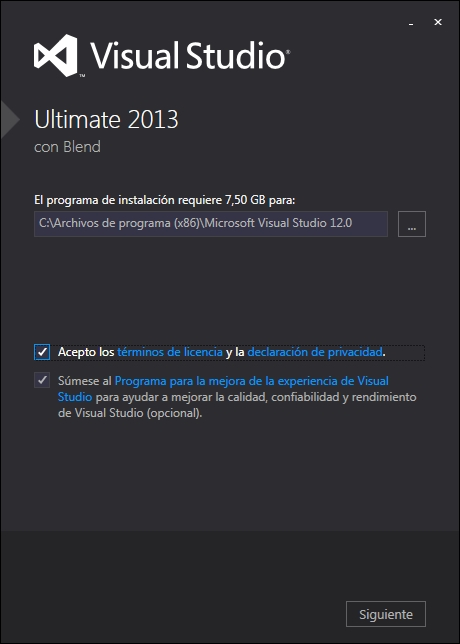
\includegraphics[width=.8\linewidth]{./img/vs-instalacion1.jpg}
\caption[]{Inicio de instalaci\'{o}n de Visual Studio\label{fig:vs-instalacion1}}
\end{figure}

\vfill

\newpage
Deje todas las opciones por defecto de <<Caracter\'{i}sticas opcionales para instalar:>> y haga click en el bot\'{o}n <<INSTALAR>> (v\'{e}ase la figura \ref{fig:vs-instalacion2}).	

\vfill

\begin{figure}[H]
  \centering
  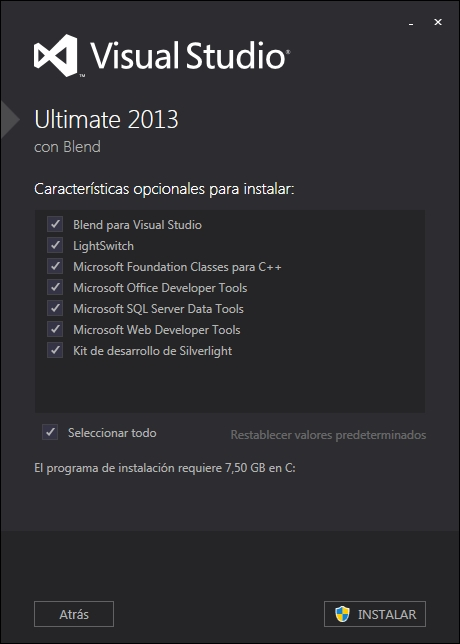
\includegraphics[width=.8\linewidth]{./img/vs-instalacion2.jpg}
\caption[]{Caracter\'{i}sticas opcionales de Visual Studio\label{fig:vs-instalacion2}}
\end{figure}

\vfill

\newpage
Espere a que el proceso de instalaci\'{o}n finalice (v\'{e}ase la figura \ref{fig:vs-instalacion3}).	

\vfill

\begin{figure}[H]
  \centering
  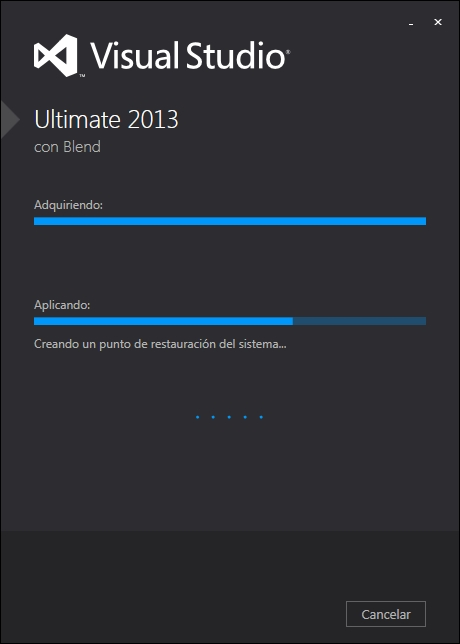
\includegraphics[width=.8\linewidth]{./img/vs-instalacion3.jpg}
\caption[]{Progreso de la instalaci\'{o}n de Visual Studio\label{fig:vs-instalacion3}}
\end{figure}

\vfill

\newpage
Despu\'{e}s de finalizar la instalaci\'{o}n, no inicie Visual Studio, haga click en el bot\'{o}n con forma de equis (x) en la esquina superior para cerrar la ventana (v\'{e}ase la figura \ref{fig:vs-instalacion4}).	

\vfill

\begin{figure}[H]
  \centering
  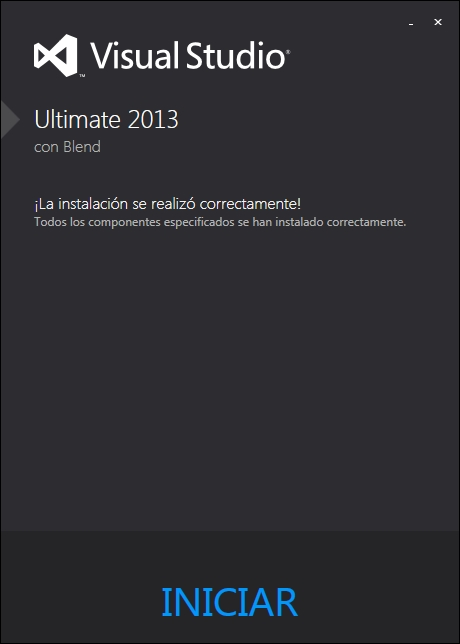
\includegraphics[width=.8\linewidth]{./img/vs-instalacion4.jpg}
\caption[]{Cerrar ventana de instalaci\'{o}n de Visual Studio\label{fig:vs-instalacion4}}
\end{figure}

\vfill

\newpage

\section*{Instalaci\'{o}n de PostgreSQL}
	
Ejecute la instalaci\'{o}n de PostgreSQL como administrador. Haga click en el bot\'{o}n <<Siguiente>> (v\'{e}ase la figura \ref{fig:postgres1}).

\vfill
\begin{figure}[H]
  \centering
  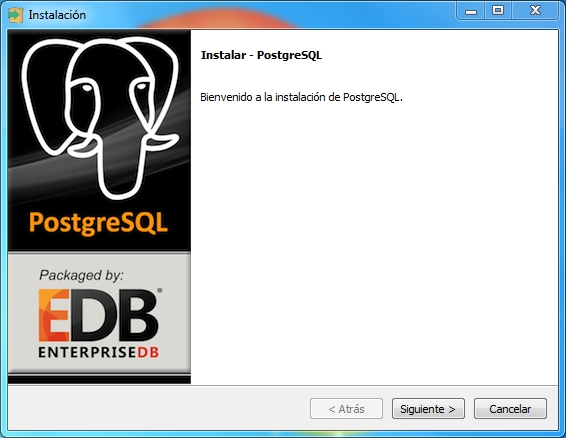
\includegraphics[width=.6\linewidth]{./img/postgres1.jpg}
\caption[]{Inicio de instalaci\'{o}n de PostgreSQL\label{fig:postgres1}}
\end{figure}
\vfill
Deje la ubicaci\'{o}n del directorio de instalaci\'{o}n por defecto y haga click en el bot\'{o}n <<Siguiente>> (v\'{e}ase la figura \ref{fig:postgres2}).
\vfill
\begin{figure}[H]
  \centering
  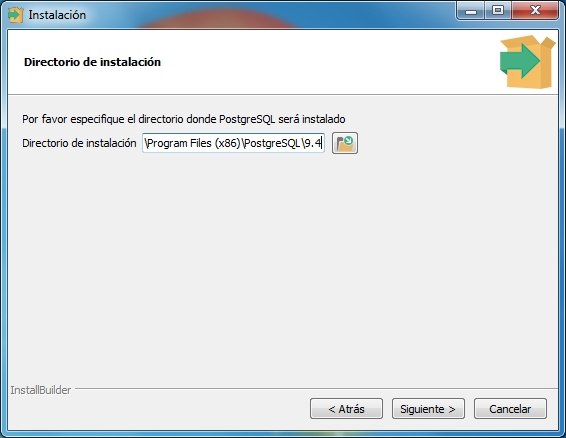
\includegraphics[width=.6\linewidth]{./img/postgres2.jpg}
\caption[]{Directorio de instalaci\'{o}n de PostgreSQL\label{fig:postgres2}}
\end{figure}
\vfill
\newpage

Deje la ubicaci\'{o}n del directorio de datos por defecto y haga click en el bot\'{o}n <<Siguiente>> (v\'{e}ase la figura \ref{fig:postgres3}).
\vfill
\begin{figure}[H]
  \centering
  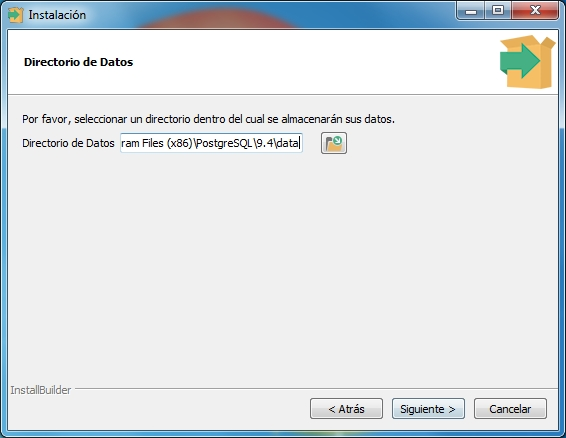
\includegraphics[width=.6\linewidth]{./img/postgres3.jpg}
\caption[]{Inicio de datos de PostgreSQL\label{fig:postgres3}}
\end{figure}
\vfill
Introduzca una contrase\~{n}a de su preferencia, gu\'{a}rdela en un lugar seguro y haga click en el bot\'{o}n <<Siguiente>> (v\'{e}ase la figura \ref{fig:postgres4}).
\vfill
\begin{figure}[H]
  \centering
  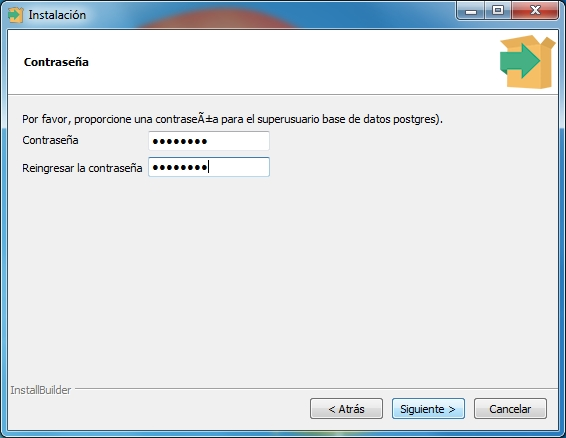
\includegraphics[width=.6\linewidth]{./img/postgres4.jpg}
\caption[]{Contrase\~{n}a para el superusuario de PostgreSQL\label{fig:postgres4}}
\end{figure}
\vfill
\newpage

Deje el n\'{u}mero del puerto por defecto y haga click en el bot\'{o}n <<Siguiente>> (v\'{e}ase la figura \ref{fig:postgres5}).
\vfill
\begin{figure}[H]
  \centering
  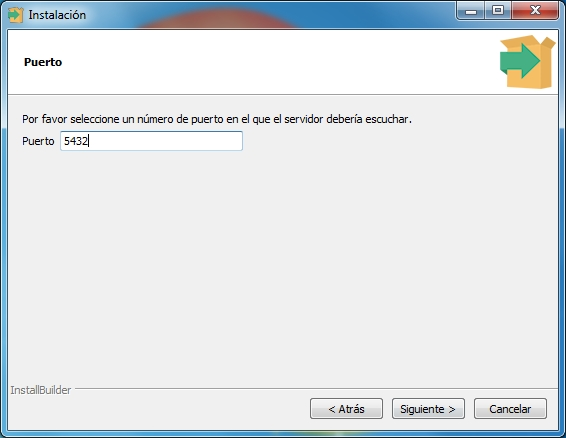
\includegraphics[width=.6\linewidth]{./img/postgres5.jpg}
\caption[]{N\'{u}mero de puerto para PostgreSQL\label{fig:postgres5}}
\end{figure}
\vfill
Deje la configuraci\'{o}n regional por defecto y haga click en el bot\'{o}n <<Siguiente>> (v\'{e}ase la figura \ref{fig:postgres6}).
\vfill
\begin{figure}[H]
  \centering
  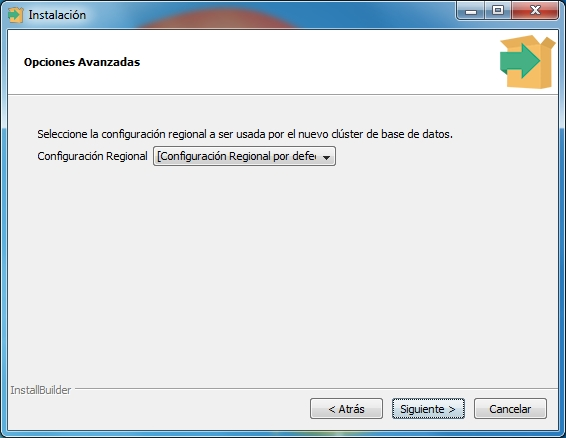
\includegraphics[width=.6\linewidth]{./img/postgres6.jpg}
\caption[]{Configuraci\'{o}n regional para PostgreSQL\label{fig:postgres6}}
\end{figure}
\vfill
\newpage

Haga click en el bot\'{o}n <<Siguiente>> para empezar el proceso de instalaci\'{o}n y espere a que finalice (v\'{e}ase las figuras \ref{fig:postgres7} y \ref{fig:postgres8}).
\vfill
\begin{figure}[H]
  \centering
  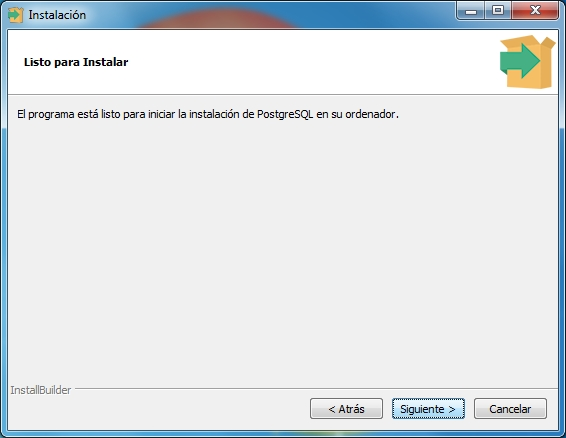
\includegraphics[width=.7\linewidth]{./img/postgres7.jpg}
\caption[]{Inicio de la instalaci\'{o}n de PostgreSQL\label{fig:postgres7}}
\end{figure}
\vfill
\begin{figure}[H]
  \centering
  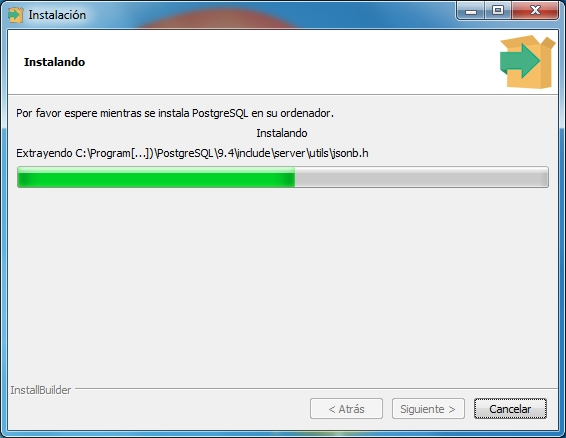
\includegraphics[width=.7\linewidth]{./img/postgres8.jpg}
\caption[]{Proceso de instalaci\'{o}n de PostgreSQL\label{fig:postgres8}}
\end{figure}
\vfill
\newpage

Despu\'{e}s de finalizar la instalaci\'{o}n, aseg\'{u}rese de que la opci\'{o}n <<Lanzar Stack Builder al finalizar>> no est\'{e} seleccionada, y por \'{u}ltimo haga click en el bot\'{o}n <<Terminar>> (v\'{e}ase la figura \ref{fig:vs-instalacion9}).	
\vfill
\begin{figure}[H]
  \centering
  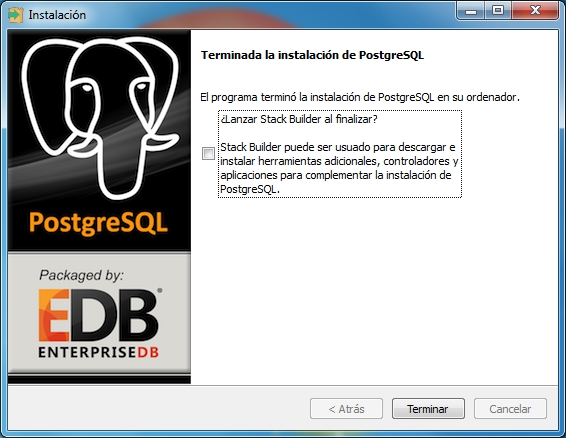
\includegraphics[width=.8\linewidth]{./img/postgres9.jpg}
\caption[]{Finalizaci\'{o}n de la instalaci\'{o}n de PostgreSQL\label{fig:vs-instalacion9}}
\end{figure}
\vfill
\newpage

\section*{Configuraci\'{o}n de Visual Studio}
	
	Ejecute el software Visual Studio como administrador. En caso de que al iniciar se le pregunte si desea iniciar sesi\'{o}n, elija la opci\'{o}n <<De momento no, quiz\'{a}s m\'{a}s tarde>> (v\'{e}ase la figura \ref{fig:vs-inicio}).	
\vfill
\begin{figure}[H]
  \centering
  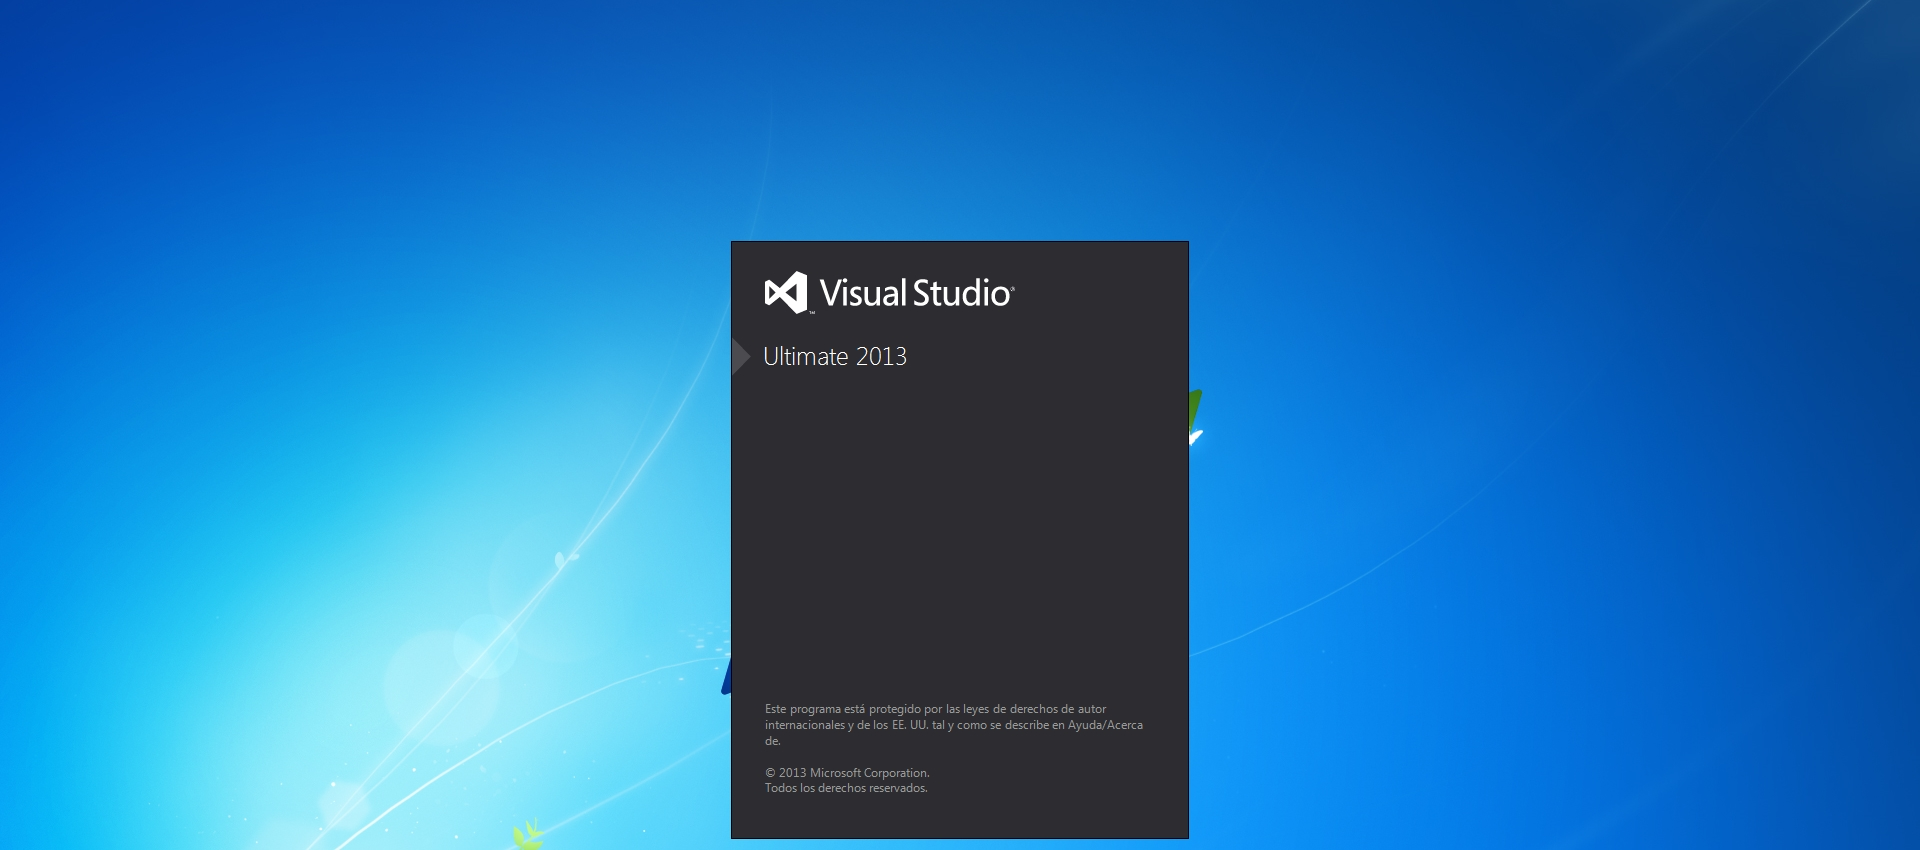
\includegraphics[width=.8\linewidth]{./img/vs-inicio.jpg}
\caption[]{Vista de inicio de Visual Studio\label{fig:vs-inicio}}
\end{figure}
\vfill
En el men\'{u} <<ARCHIVO>> entre al submen\'{u} <<Abrir>> y haga click en la opci\'{o}n <<Proyecto o soluci\'{o}n...>> (v\'{e}ase la figura \ref{fig:vs-abrir}).	
\vfill
\begin{figure}[H]
  \centering
  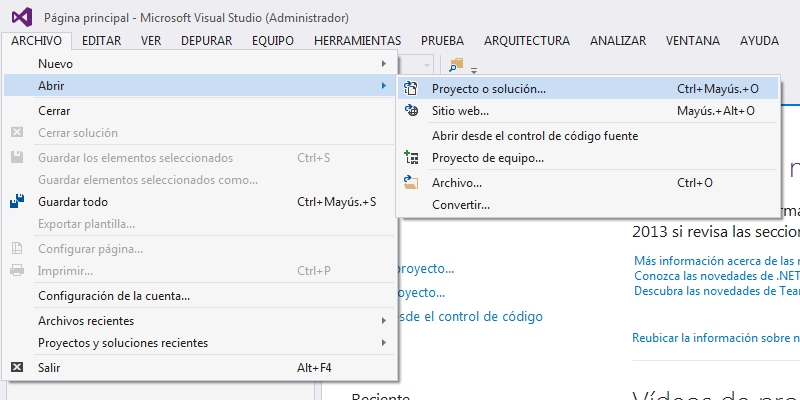
\includegraphics[width=.8\linewidth]{./img/vs-proyecto-abrir.jpg}
\caption[]{Abrir proyecto\label{fig:vs-abrir}}
\end{figure}
\vfill
\newpage

En la carpeta <<MSXEBridge>> ubicada en el disco <<C:\textbackslash>>, seleccione el archivo <<MSXEBridge>> y haga click en el bot\'{o}n <<Abrir>> (v\'{e}ase la figura \ref{fig:vs-abrir-buscar}).
\vfill
\begin{figure}[H]
  \centering
  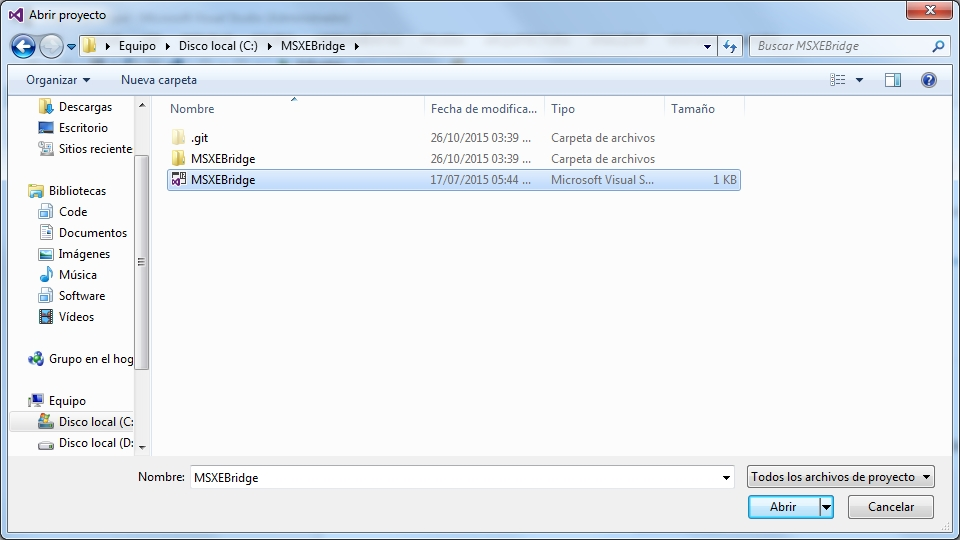
\includegraphics[width=.8\linewidth]{./img/vs-abrir-buscar.jpg}
\caption[]{Buscar el archivo MSXEBridge\label{fig:vs-abrir-buscar}}
\end{figure}
\vfill
En la parte derecha de Visual Studio, haga click con el bot\'{o}n derecho en <<MSXEBridge>> y seleccione la opci\'{o}n <<Propiedades>> (v\'{e}ase la figura \ref{fig:vs-propiedades}).
\vfill
\begin{figure}[H]
  \centering
  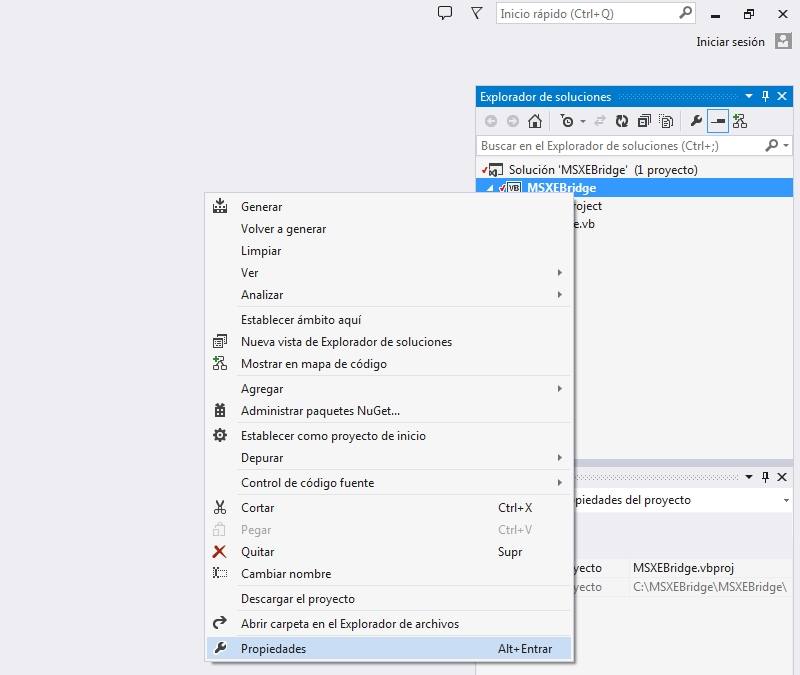
\includegraphics[width=.7\linewidth]{./img/vs-propiedades.jpg}
\caption[]{Propiedades de MSXEBridge\label{fig:vs-propiedades}}
\end{figure}
\vfill
\newpage

Haga click al bot\'{o}n <<Informaci\'{o}n de ensamblado...>>, aseg\'{u}rese de que la opci\'{o}n <<Crear ensamblado visible a trav\'{e}s de COM>> est\'{e} seleccionada, y haga click en el bot\'{o}n <<Aceptar>> (v\'{e}ase la figura \ref{fig:vs-ensamblado}).
\vfill
\begin{figure}[H]
  \centering
  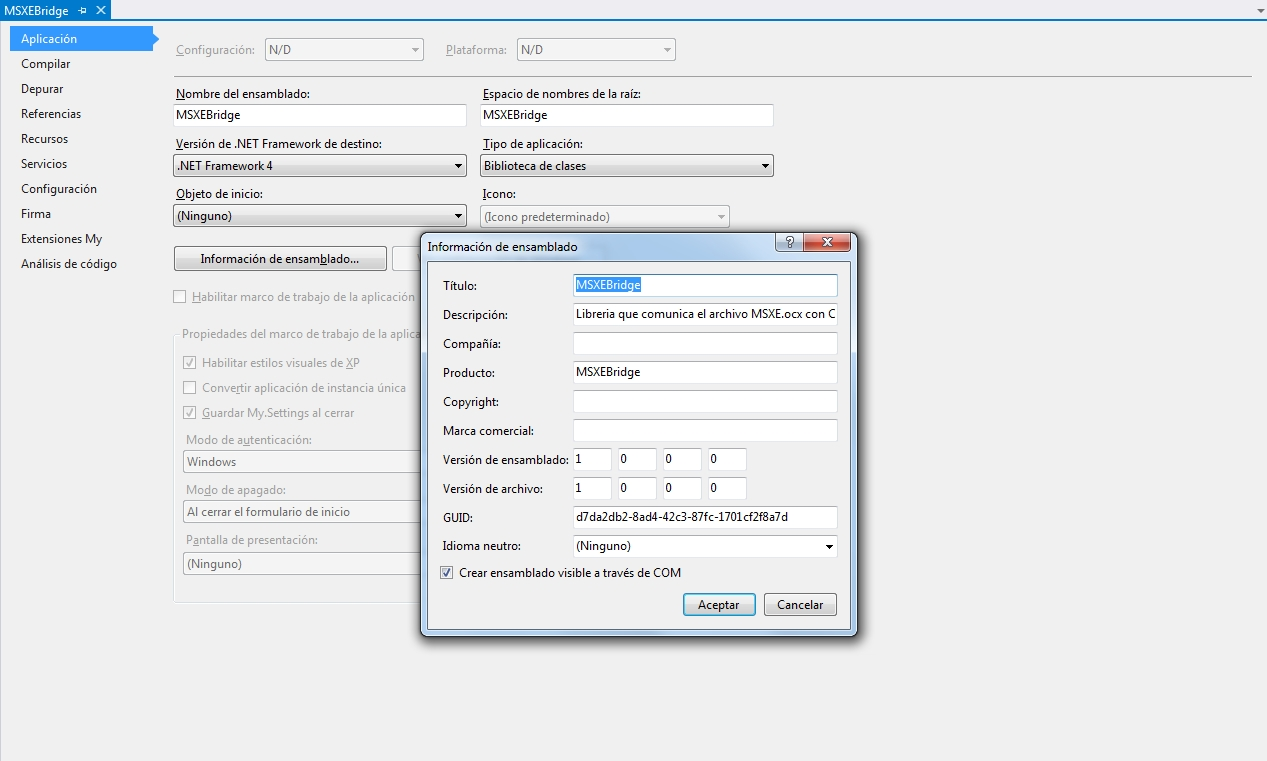
\includegraphics[width=.75\linewidth]{./img/vs-ensamblado.jpg}
\caption[]{Ensamblado de MSXEBridge\label{fig:vs-ensamblado}}
\end{figure}
\vfill
Haga click en la pesta\~{n}a <<Compilar>> y aseg\'{u}rese de que la opci\'{o}n <<Registrar para interoperabilidad COM>> est\'{e} seleccionada (v\'{e}ase la figura \ref{fig:vs-compilar}).
\vfill
\begin{figure}[H]
  \centering
  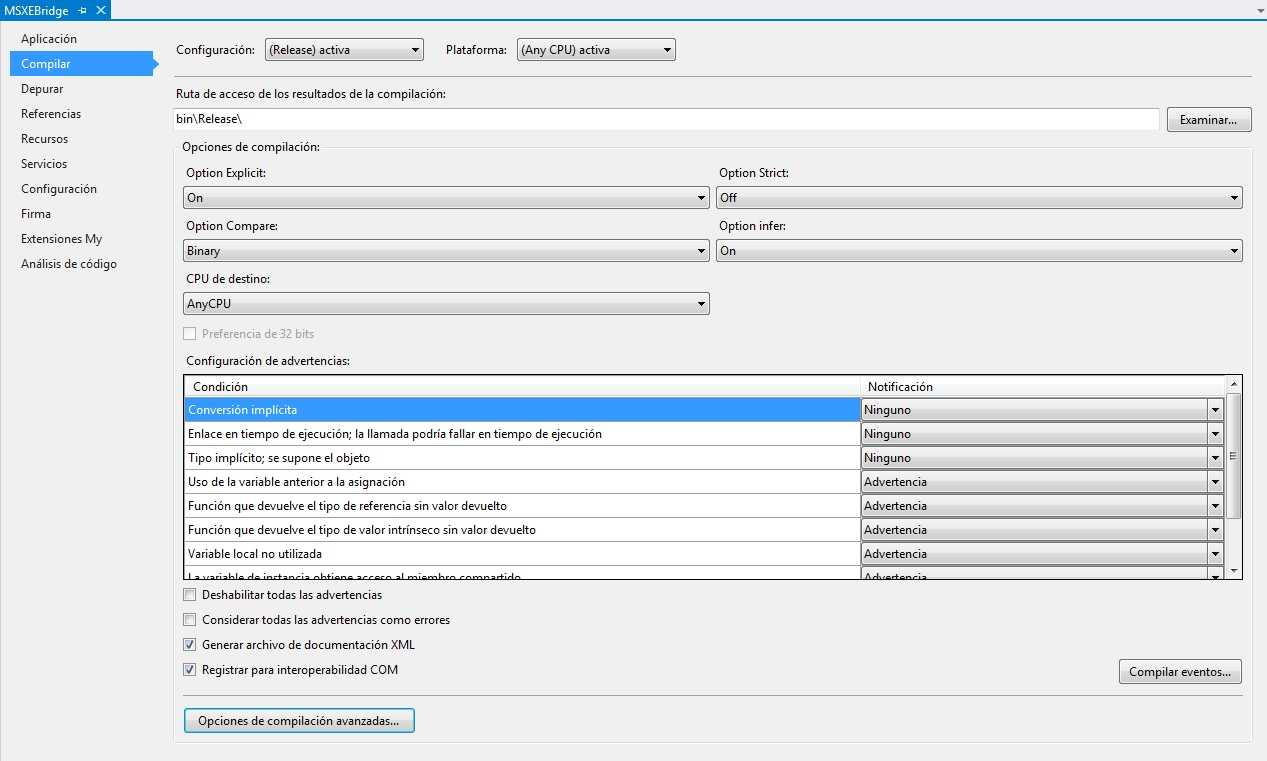
\includegraphics[width=.75\linewidth]{./img/vs-compilar.jpg}
\caption[]{Interoperabilidad de MSXEBridge\label{fig:vs-compilar}}
\end{figure}
\vfill
\newpage

En el men\'{u} <<COMPILAR>>, haga click en la opci\'{o}n <<Compilar soluci\'{o}n>> (v\'{e}ase la figura \ref{fig:vs-compilar-solucion}).
\vfill
\begin{figure}[H]
  \centering
  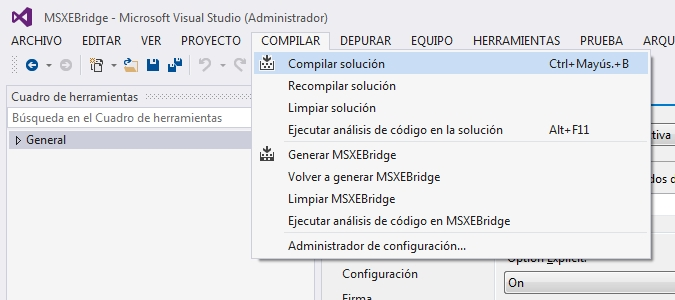
\includegraphics[width=1\linewidth]{./img/vs-compilar-solucion.jpg}
\caption[]{Compilar MSXEBridge\label{fig:vs-compilar-solucion}}
\end{figure}
\vfill
En la parte inferior de Visual Studio podr\'{a} ver que la compilaci\'{o}n finaliz\'{o} correctamente (v\'{e}ase la figura \ref{fig:vs-resultados}). Por \'{u}ltimo, cierre el software Visual Studio.
\vfill
\begin{figure}[H]
  \centering
  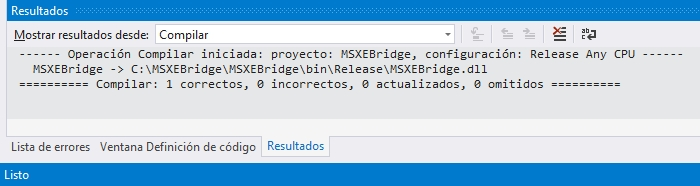
\includegraphics[width=1\linewidth]{./img/vs-resultados.jpg}
\caption[]{Resultados de la compilaci\'{o}n\label{fig:vs-resultados}}
\end{figure}
\vfill
Es importante destacar que los pasos seguidos previamente s\'{o}lo se deben realizar una vez, y no es necesario que ejecute Visual Studio posteriormente para ejecutar el Spectrasoft.

\newpage

\section*{Configuraci\'{o}n de PostgreSQL}
	
Ejecute el software pgAdmin como administrador (v\'{e}ase la figura \ref{fig:pgadmin-inicio}).
\vfill
\begin{figure}[H]
  \centering
  
\includegraphics[width=1\linewidth]{./img/pgadmin-inicio.jpg}
\caption[]{Vista de inicio de pgAdmin\label{fig:pgadmin-inicio}}
\end{figure}
\vfill
Para accesar al servidor, haga doble click en la opci\'{o}n <<PostgreSQL (localhost:5432)>>, e introduzca la contrase\~{n}a que estableci\'{o} durante el proceso de instalaci\'{o}n (v\'{e}ase la figura \ref{fig:pgadmin-acceso}).
\vfill
\begin{figure}[H]
  \centering
  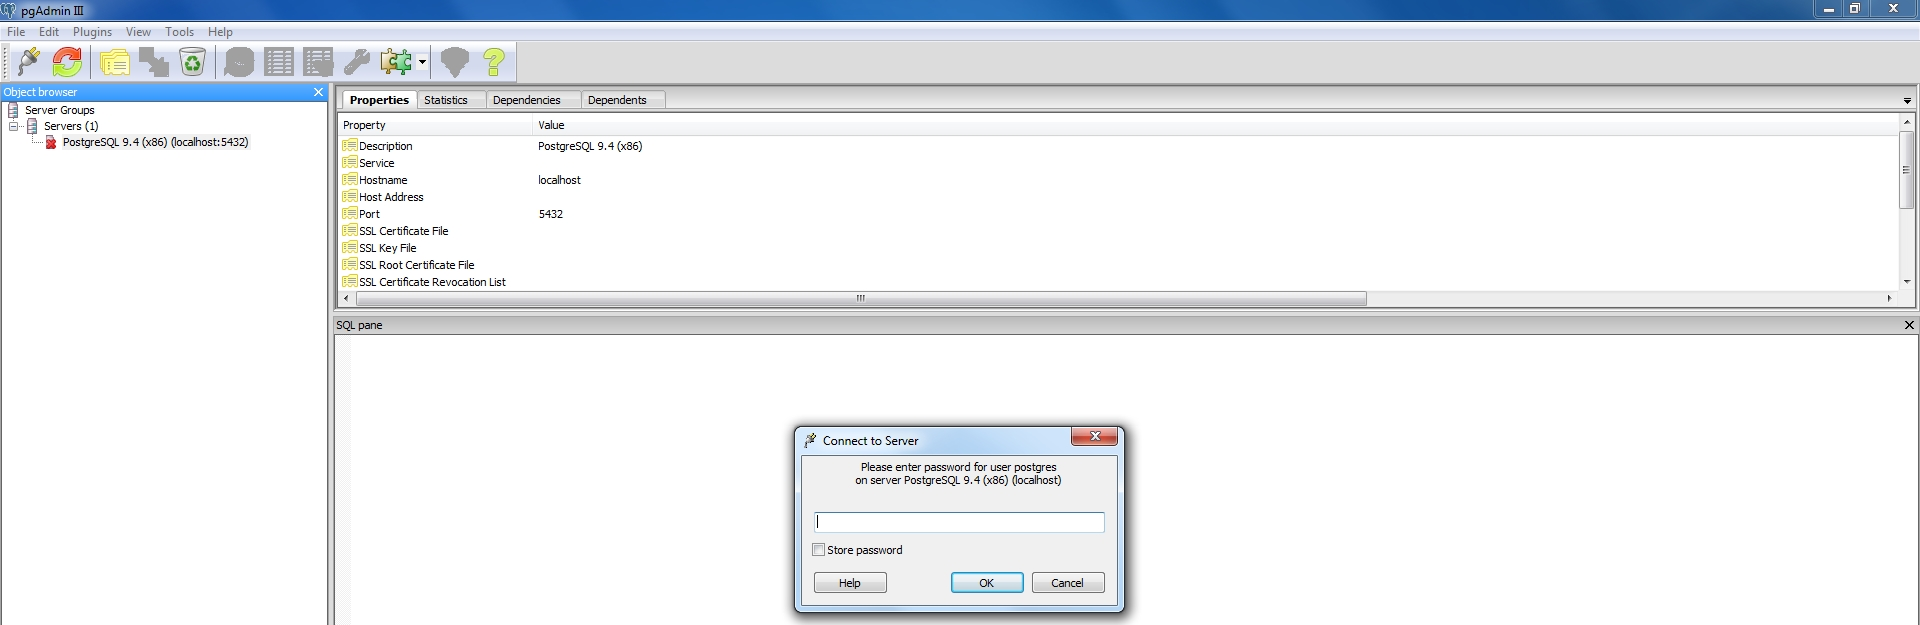
\includegraphics[width=1\linewidth]{./img/pgadmin-acceso.jpg}
\caption[]{Acceso al servidor\label{fig:pgadmin-acceso}}
\end{figure}
\vfill
\newpage

Haga click derecho en el men\'{u} <<Login Roles>> y seleccione la opci\'{o}n <<New Login Role...>> (v\'{e}ase la figura \ref{fig:pgadmin-rol}).
\vfill
\begin{figure}[H]
  \centering
  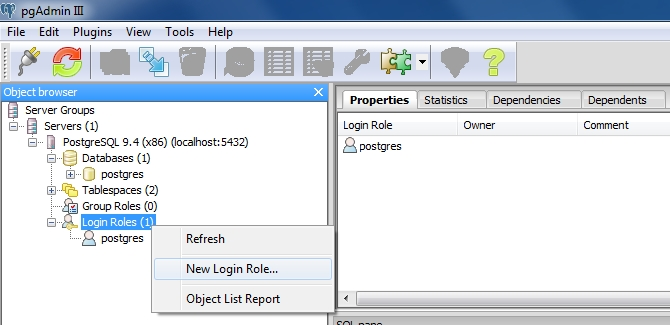
\includegraphics[width=1\linewidth]{./img/pgadmin-rol.jpg}
\caption[]{Crear nuevo rol\label{fig:pgadmin-rol}}
\end{figure}
\vfill
Introduzca <<CIMBUC>> en <<Role name>> (v\'{e}ase la figura \ref{fig:pgadmin-rol-nombre}).
\vfill
\begin{figure}[H]
  \centering
  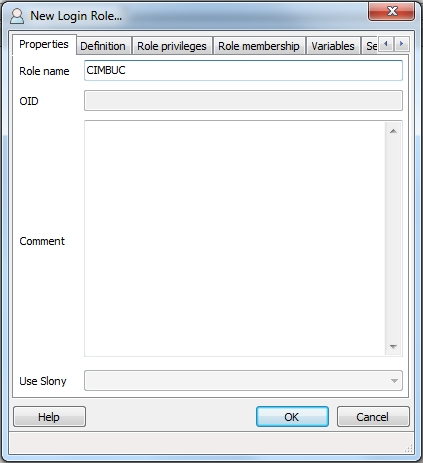
\includegraphics[width=.5\linewidth]{./img/pgadmin-rol-nombre.jpg}
\caption[]{Nombre del rol\label{fig:pgadmin-rol-nombre}}
\end{figure}
\vfill
Haga click en la pesta\~{n}a <<Definition>> e introduzca <<CIMBUC>> como la contrase\~{n}a del rol (v\'{e}ase la figura \ref{fig:pgadmin-rol-clave}).
\vfill
\begin{figure}[H]
  \centering
  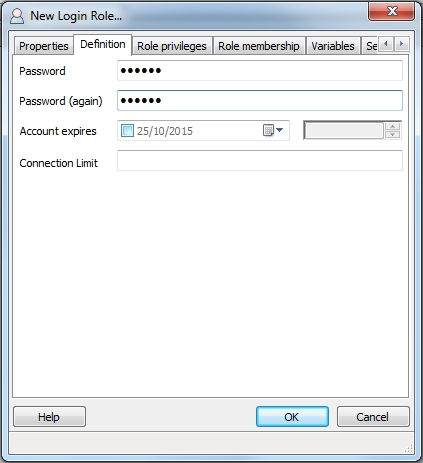
\includegraphics[width=.45\linewidth]{./img/pgadmin-rol-clave.jpg}
\caption[]{Contrase\~{n}a del rol\label{fig:pgadmin-rol-clave}}
\end{figure}
\vfill
Haga click en la pesta\~{n}a <<Role privileges>>, seleccione todas las opciones de privilegios disponibles para el rol y haga click en el bot\'{o}n <<OK>> (v\'{e}ase la figura \ref{fig:pgadmin-rol-privilegios}).
\vfill
\begin{figure}[H]
  \centering
  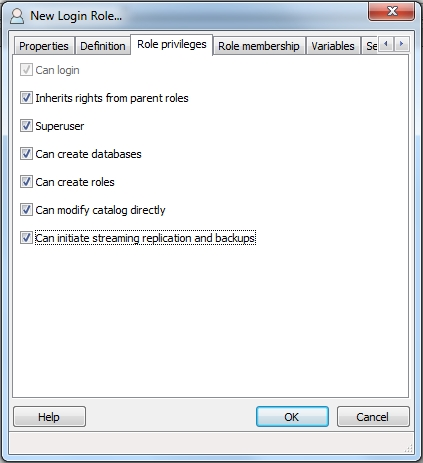
\includegraphics[width=.45\linewidth]{./img/pgadmin-rol-privilegios.jpg}
\caption[]{Privilegios del rol\label{fig:pgadmin-rol-privilegios}}
\end{figure}
\vfill
\newpage

Haga click derecho en el men\'{u} <<Databases>> y seleccione la opci\'{o}n <<New Database...>> (v\'{e}ase la figura \ref{fig:pgadmin-bd}).
\vfill
\begin{figure}[H]
  \centering
  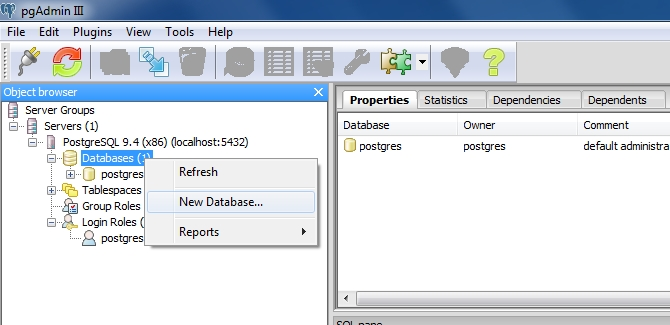
\includegraphics[width=1\linewidth]{./img/pgadmin-bd.jpg}
\caption[]{Crear nueva base de datos\label{fig:pgadmin-bd}}
\end{figure}
\vfill
Introduzca <<CIMBUC>> en <<Name>> y haga click en el bot\'{o}n <<OK>> (v\'{e}ase la figura \ref{fig:pgadmin-bd-nombre}).
\vfill
\begin{figure}[H]
  \centering
  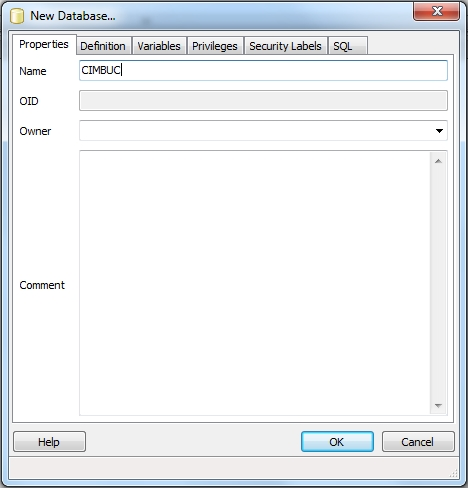
\includegraphics[width=.5\linewidth]{./img/pgadmin-bd-nombre.jpg}
\caption[]{Nombre de la base de datos\label{fig:pgadmin-bd-nombre}}
\end{figure}
\vfill
\newpage

Haga click derecho en la base de datos <<CIMBUC>> y seleccione la opci\'{o}n <<Restore...>> (v\'{e}ase la figura \ref{fig:pgadmin-restaurar}).
\vfill
\begin{figure}[H]
  \centering
  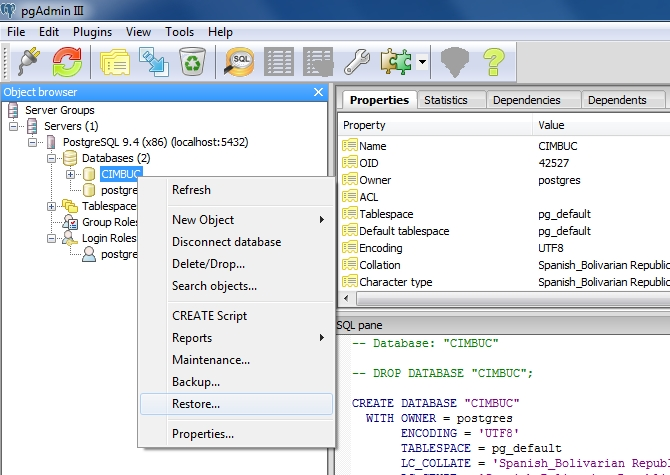
\includegraphics[width=1\linewidth]{./img/pgadmin-restaurar.jpg}
\caption[]{Opci\'{o}n de restauraci\'{o}n de la base de datos\label{fig:pgadmin-restaurar}}
\end{figure}
\vfill
\newpage

Haga click en el bot\'{o}n <<...>> para buscar el archivo de respaldo de la base de datos (v\'{e}ase la figura \ref{fig:pgadmin-restaurar-ventana}).
\vfill
\begin{figure}[H]
  \centering
  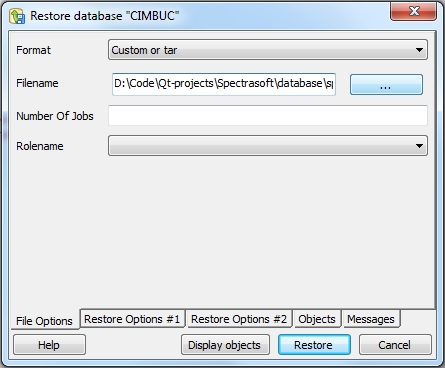
\includegraphics[width=.6\linewidth]{./img/pgadmin-restaurar-ventana.jpg}
\caption[]{Ventana de restauraci\'{o}n de la base de datos\label{fig:pgadmin-restaurar-ventana}}
\end{figure}
\vfill
En la carpeta con los paquetes de instalaci\'{o}n, busque y seleccione el archivo <<spectradb.backup>>, y haga click en el bot\'{o}n <<Abrir>> (v\'{e}ase la figura \ref{fig:pgadmin-restaurar-buscar}).
\vfill
\begin{figure}[H]
  \centering
  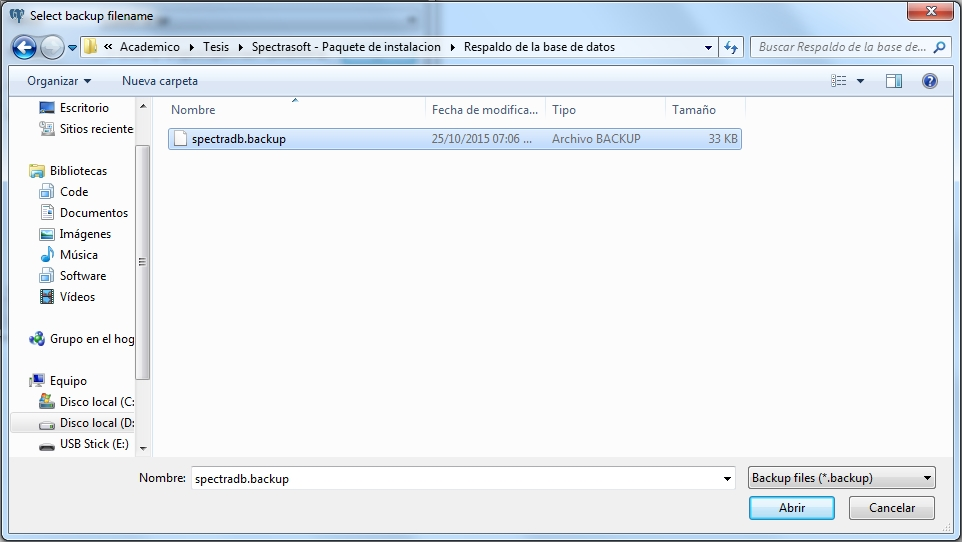
\includegraphics[width=1\linewidth]{./img/pgadmin-restaurar-buscar.jpg}
\caption[]{Buscar el archivo de respaldo\label{fig:pgadmin-restaurar-buscar}}
\end{figure}
\vfill
\newpage

De vuelta a la ventana de restauraci\'{o}n, haga click en la lista desplegable de <<Rolename>> y seleccione la opci\'{o}n <<CIMBUC>> (v\'{e}ase la figura \ref{fig:pgadmin-restaurar-rol}).
v
\begin{figure}[H]
  \centering
  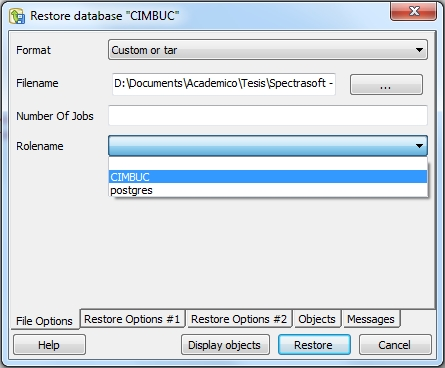
\includegraphics[width=.6\linewidth]{./img/pgadmin-restaurar-rol.jpg}
\caption[]{Rol de restauraci\'{o}n de la base de datos\label{fig:pgadmin-restaurar-rol}}
\end{figure}
\vfill
Haga click en la pesta\~{n}a <<Restore Options \#1>> y en el grupo <<Sections>> seleccione las opciones <<Pre-data>>, <<Data>> y <<Post-data>>, luego haga click en el bot\'{o}n <<Restore>> (v\'{e}ase la figura \ref{fig:pgadmin-restaurar-opciones}).
\vfill
\begin{figure}[H]
  \centering
  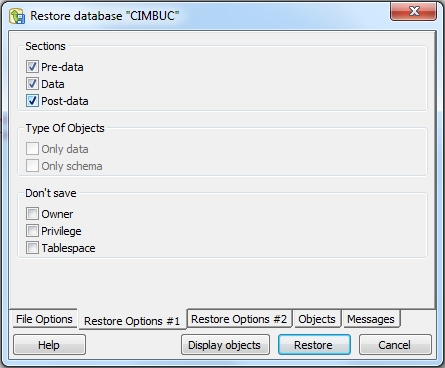
\includegraphics[width=.6\linewidth]{./img/pgadmin-restaurar-opciones.jpg}
\caption[]{Opciones de restauraci\'{o}n de la base de datos\label{fig:pgadmin-restaurar-opciones}}
\end{figure}
\vfill
\newpage

En la misma ventana haga click en bot\'{o}n <<Done>>, y por \'{u}ltimo cierre el software pgAdmin (v\'{e}ase la figura \ref{fig:pgadmin-restaurar-listo}).
\vfill
\begin{figure}[H]
  \centering
  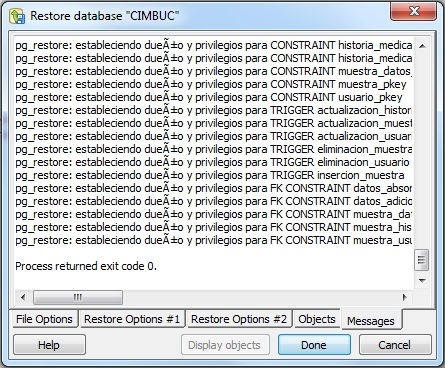
\includegraphics[width=.6\linewidth]{./img/pgadmin-restaurar-listo.jpg}
\caption[]{Restauraci\'{o}n de la base de datos completa\label{fig:pgadmin-restaurar-listo}}
\end{figure}
\vfill
Es importante destacar que los pasos seguidos previamente s\'{o}lo se deben realizar una vez, y no es necesario que ejecute pgAdmin posteriormente para ejecutar el Spectrasoft.

La base de datos posee un usuario administrador por defecto para iniciar sesi\'{o}n y trabajar con el Spectrasoft, sus datos de ingreso son los siguientes: 
\vfill
\begin{itemize}
	\item \textbf{C\'{e}dula de identidad:} V00000000
	
	\item \textbf{Contrase\~{n}a:} 12345Admin
\end{itemize}
\vfill
Luego de iniciar sesi\'{o}n en el Spectrasoft con este usuario, puede crear otro usuario administrador de su preferencia y eliminar \'{e}ste.

\section*{Instalaci\'{o}n del Spectrasoft}

Ejecute el instalador <<setup-spectrasoft>> y haga click en el bot\'{o}n <<Next>>, dejando todas las opciones por defecto hasta llegar al acuerdo de licencia (v\'{e}ase la figura \ref{fig:spectrasoft-setup}).
\vfill
\begin{figure}[H]
  \centering
  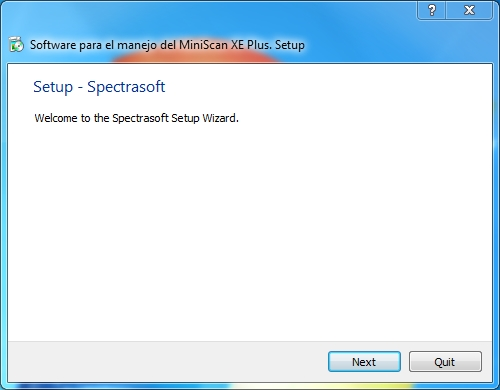
\includegraphics[width=.5\linewidth]{./img/spectrasoft-setup.jpg}
\caption[]{Instalador del Spectrasoft\label{fig:spectrasoft-setup}}
\end{figure}
\vfill
En la ventana <<License Agreement>>, seleccione la opci\'{o}n <<I accept the license>> y haga click en el bot\'{o}n <<Next>> (v\'{e}ase la figura \ref{fig:spectrasoft-licencia}). Deje las siguientes opciones por defecto hasta llegar la opci\'{o}n de instalar.
\vfill
\begin{figure}[H]
  \centering
  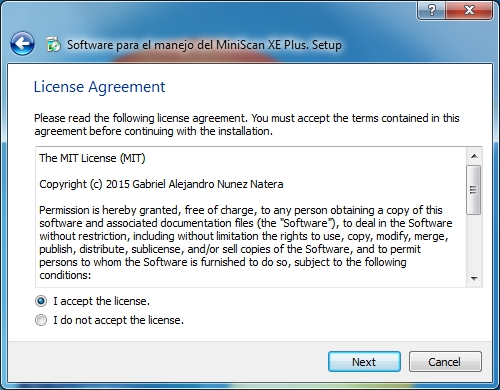
\includegraphics[width=.5\linewidth]{./img/spectrasoft-licencia.jpg}
\caption[]{Licencia del Spectrasoft\label{fig:spectrasoft-licencia}}
\end{figure}
\vfill
\newpage

En la ventana <<Ready to Install>> haga click en el bot\'{o}n <<Install>> (v\'{e}ase la figura \ref{fig:spectrasoft-instalar}).
\vfill
\begin{figure}[H]
  \centering
  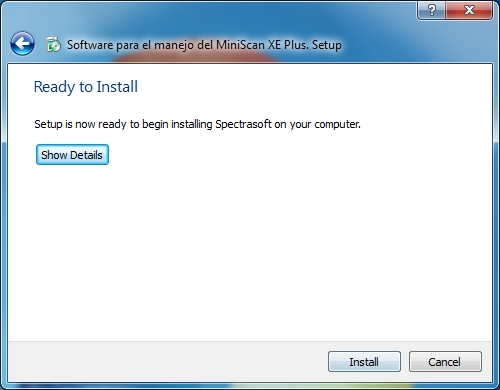
\includegraphics[width=.6\linewidth]{./img/spectrasoft-instalar.jpg}
\caption[]{Instalar el Spectrasoft\label{fig:spectrasoft-instalar}}
\end{figure}
\vfill
En la ventana <<Completing the Spectrasoft Wizard>> haga click en el bot\'{o}n <<Finish>> (v\'{e}ase la figura \ref{fig:spectrasoft-finalizar}).
\vfill
\begin{figure}[H]
  \centering
  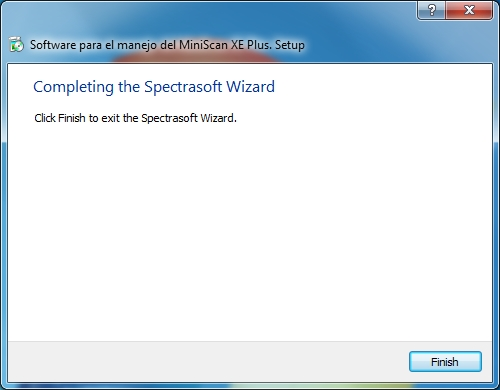
\includegraphics[width=.6\linewidth]{./img/spectrasoft-finalizar.jpg}
\caption[]{Finalizar la instalaci\'{o}n\label{fig:spectrasoft-finalizar}}
\end{figure}
\vfill
\newpage

Por \'{u}ltimo, para ejecutar el Spectrasoft abra el men\'{u} de inicio de Windows y haga click en la opci\'{o}n <<Spectrasoft>> (v\'{e}ase la figura \ref{fig:spectrasoft-ejecutable}).
\vfill
\begin{figure}[H]
  \centering
  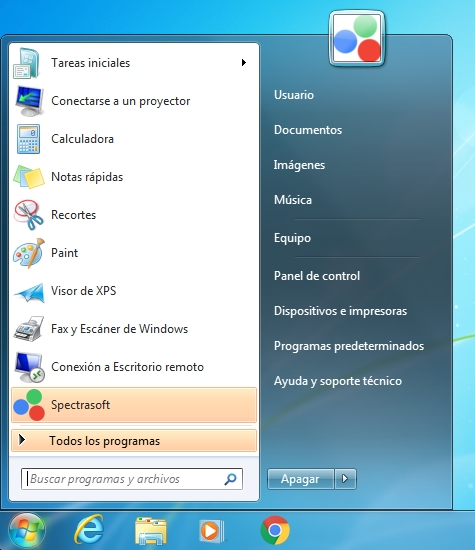
\includegraphics[width=.4\linewidth]{./img/spectrasoft-ejecutable.jpg}
\caption[]{Ejecutar el Spectrasoft\label{fig:spectrasoft-ejecutable}}
\end{figure}
\vfill
Si desea entrar al men\'{u} del Spectrasoft, abra el men\'{u} de inicio de Windows, haga click en la opci\'{o}n <<Todos los programas>>, busque la carpeta llamada <<Spectrasoft>> y seleccionela (v\'{e}ase la figura \ref{fig:spectrasoft-menu}).
\vfill
\begin{figure}[H]
  \centering
  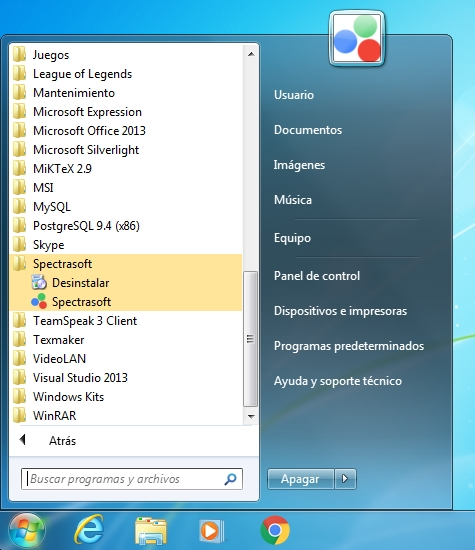
\includegraphics[width=.4\linewidth]{./img/spectrasoft-menu.jpg}
\caption[]{Men\'{u} del Spectrasoft\label{fig:spectrasoft-menu}}
\end{figure}
\vfill
\newpage
%%%%%%%%%%%%%%%%%%%%%%
%%%%%%%%%%%%%%%%%%%%%%
\chapter{Manual de usuario}
\thispagestyle{fancy}

\begin{center}
	
\includegraphics[width=0.10\textwidth]{./img/logo.png}
\end{center}

\vfill
\section*{Introducci\'{o}n}
	El Spectrasoft es un software de c\'{o}digo abierto para el manejo del MiniScan XE Plus, el cual es usado en el diagn\'{o}stico de patolog\'{i}as dermatol\'{o}gicas en pacientes. Este software ofrece funciones de gesti\'{o}n de mediciones, historias m\'{e}dicas de pacientes y muestras. La vista principal del Spectrasoft es la mostrada en la figura \ref{fig:vista-principal}.
\vfill
\begin{figure}[H]
  \centering
  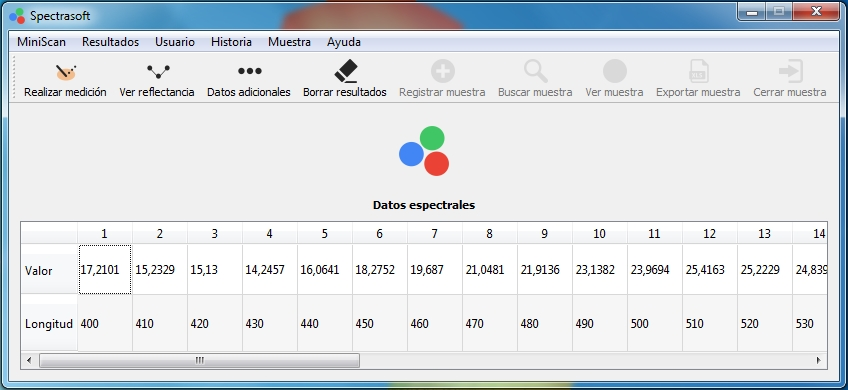
\includegraphics[width=1\linewidth]{./img/vista-principal.jpg}
\caption[]{Vista principal del Spectrasoft\label{fig:vista-principal}}
\end{figure}
\vfill
\newpage

\section*{Permisolog\'{i}a de los usuarios}

	Spectrasoft maneja tres roles de usuario: administradores, dermat\'{o}logos e investigadores. Si bien los tres roles comparten acciones comunes que pueden realizar, cada uno tiene permisos diferentes que lo distinguen de los dem\'{a}s. Estos permisos son descritos en la tabla 1.

\begin{table}[h]
		\small
		\caption[]{Permisolog\'{i}a de los usuarios}
		\centering
		\setlength{\extrarowheight}{\altocelda}
		\begin{tabulary}{\anchotabla}{|c|J|}
			\hline
			\thead{\textbf{\small{Usuario}}} & \thead{\textbf{\small{Permisos}}}\\ \hline
			
			\textbf{Administrador} &
			
			Manejar el MiniScan XE Plus.
			
			Registrar, buscar, modificar y eliminar usuarios.
			
			Buscar y ver historias m\'{e}dicas de pacientes.
			
			Buscar y ver muestras de pacientes.\\ \hline
			
			\textbf{Dermat\'{o}logo} &
			
			Manejar el MiniScan XE Plus.
			
			Registrar, buscar, ver, modificar y eliminar historias m\'{e}dicas de pacientes.
			
			Registrar, buscar, ver, modificar y eliminar muestras de pacientes.\\ \hline
			
			\textbf{Investigador} &
			
			Manejar el MiniScan XE Plus.
			
			Buscar y ver historias m\'{e}dicas de pacientes.
			
			Buscar y ver muestras de pacientes.\\ \hline
		\end{tabulary}
	\end{table}

	Es importante destacar que todas las operaciones de registro, modificaci\'{o}n y eliminaci\'{o}n requieren de la contrase\~{n}a del usuario responsable de dicha operaci\'{o}n.
	
\newpage

\section*{Manejo del MiniScan XE Plus}

	\subsection*{Conectar y desconectar}
		Para conectar o desconectar el MiniScan XE Plus, entre al men\'{u} del MiniScan (v\'{e}ase la figura \ref{fig:conectar-desconectar}).
\vfill
\begin{figure}[H]
\centering
\begin{subfigure}{.5\textwidth}
  \centering
  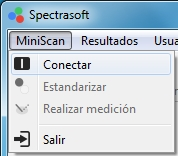
\includegraphics[width=.6\linewidth]{./img/conectar.jpg}
\end{subfigure}%
\begin{subfigure}{.5\textwidth}
  \centering
  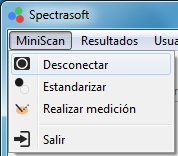
\includegraphics[width=.6\linewidth]{./img/desconectar.jpg}
\end{subfigure}
\caption[]{Conectar y desconectar MiniScan XE Plus\label{fig:conectar-desconectar}}
\end{figure}
\vfill
	\subsection*{Calibrar}
		Entre al men\'{u} del Miniscan y seleccione la opci\'{o}n estandarizar. Prepare la trampa negra del Miniscan para su medici\'{o}n y seleccione listo, por \'{u}ltimo prepare la cer\'{a}mica blanca para su medici\'{o}n y seleccione listo (v\'{e}ase la figura \ref{fig:calibrar}).
\vfill
\begin{figure}[H]
\centering
\begin{subfigure}{.33\textwidth}
  \centering
  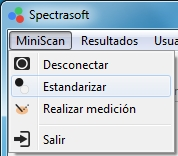
\includegraphics[width=.9\linewidth]{./img/estandarizar.jpg}
\end{subfigure}%
\centering
\begin{subfigure}{.33\textwidth}
  \centering
  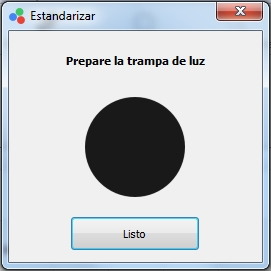
\includegraphics[width=.9\linewidth]{./img/estandarizar-negro.jpg}
\end{subfigure}%
\begin{subfigure}{.33\textwidth}
  \centering
  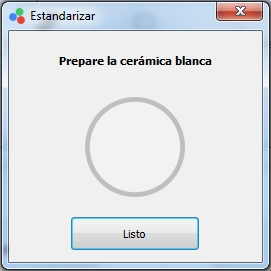
\includegraphics[width=.9\linewidth]{./img/estandarizar-blanco.jpg}
\end{subfigure}
\caption[]{Calibrar el MiniScan XE Plus\label{fig:calibrar}}
\end{figure}
\vfill
\section*{Gesti\'{o}n de mediciones}
	
	\subsection*{Realizar una medici\'{o}n}
	
	Entre al men\'{u} del MiniScan, o bien seleccione la opci\'{o}n directamente de la barra de herramientras (v\'{e}ase la figura \ref{fig:medicion}).

\begin{figure}[H]
\centering
\begin{subfigure}{.5\textwidth}
  \centering
  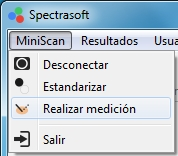
\includegraphics[width=.6\linewidth]{./img/medir-menu.jpg}
\end{subfigure}%
\begin{subfigure}{.5\textwidth}
  \centering
  \includegraphics[width=.6\linewidth]{./img/medir-barra.jpg}
\end{subfigure}
\caption[]{Realizar medici\'{o}n\label{fig:medicion}}
\end{figure}

	\subsection*{Consultar resultados de una medici\'{o}n}
	
	El men\'{u} de los resultados de una medici\'{o}n es ilustrado en la figura \ref{fig:menu-resultados}, y todos los resultados son ilustrados desde la figura \ref{fig:datos-espectrales} a la figura \ref{fig:resultados-adicionales}.

\begin{figure}[H]
  \centering
  \includegraphics[width=.5\linewidth]{./img/resultados-menu.jpg}
\caption[]{Men\'{u} de resultados de una medici\'{o}n\label{fig:menu-resultados}}
\end{figure}
\newpage
\null
\vfill
\begin{figure}[H]
  \centering
  \includegraphics[width=1\linewidth]{./img/resultados.jpg}
\caption[]{Datos espectrales de una medici\'{o}n\label{fig:datos-espectrales}}
\end{figure}
\vfill
\begin{figure}[H]
  \centering
  \includegraphics[width=1\linewidth]{./img/resultados-reflectancia.jpg}
\caption[]{Curva de reflectancia de una medici\'{o}n\label{fig:resultados-reflectancia}}
\end{figure}
\vfill
\newpage
\null
\vfill
\begin{figure}[H]
  \centering
  \includegraphics[width=1\linewidth]{./img/resultados-absorbancia.jpg}
\caption[]{Curva de absorbancia de una medici\'{o}n\label{fig:resultados-absorbancia}}
\end{figure}
\vfill
\begin{figure}[H]
  \centering
  \includegraphics[width=1\linewidth]{./img/resultados-absorcion.jpg}
\caption[]{Curva de absorci\'{o}n de una medici\'{o}n\label{fig:resultados-absorcion}}
\end{figure}
\vfill
\newpage
\null
\vfill
\begin{figure}[H]
  \centering
  \includegraphics[width=.6\linewidth]{./img/resultados-adicionales.jpg}
\caption[]{Datos adicionales de una medici\'{o}n\label{fig:resultados-adicionales}}
\end{figure}
\vfill
\newpage

\section*{Gesti\'{o}n de sesiones}

	\subsection*{Iniciar sesi\'{o}n}
	
	Para iniciar sesi\'{o}n entre al men\'{u} de usuario y seleccione la opci\'{o}n iniciar sesi\'{o}n. Debe ingresar su c\'{e}dula de identidad y su contrase\~{n}a. Esto es ilustrado en la figura \ref{fig:iniciar-sesion}.
	
\begin{figure}[H]
  \centering
  \includegraphics[width=1\linewidth]{./img/inicio-sesion.jpg}
\caption[]{Iniciar sesi\'{o}n\label{fig:iniciar-sesion}}
\end{figure}
	
	\subsection*{Ver informaci\'{o}n del usuario}
	
	Seleccione la opci\'{o}n ver usuario, ubicada en el men\'{u} de usuario. El men\'{u} de usuario y la ventana de informaci\'{o}n son ilustrados en las figuras \ref{fig:menu-usuario} y \ref{fig:ver-usuario}.
\newpage
\null
\vfill
\begin{figure}[H]
  \centering
  \includegraphics[width=.3\linewidth]{./img/menu-usuario.jpg}
\caption[]{Men\'{u} de usuario\label{fig:menu-usuario}}
\end{figure}

\begin{figure}[H]
  \centering
  \includegraphics[width=.5\linewidth]{./img/ver-usuario.jpg}
\caption[]{Ver usuario\label{fig:ver-usuario}}
\end{figure}
\vfill
\newpage

	\subsection*{Modificar informaci\'{o}n del usuario}

	Seleccione la opci\'{o}n modificar usuario, ubicada en el men\'{u} de usuario. La ventana para modificar el usuario es ilustrada en la figura \ref{fig:modificar-usuario}.

	\subsection*{Cambiar contrase\~{n}a del usuario}

	Seleccione la opci\'{o}n cambiar contrase\~{n}a, ubicada en el men\'{u} de usuario. Debe ingresar la contrase\~{n}a actual del usuario y la nueva contrase\~{n}a (dos veces) para poder realizar el cambio. La ventana para realizar esta operaci\'{o}n se ilustra en la figura \ref{fig:cambiar-clave}.

\begin{figure}[H]
\centering
\begin{minipage}{.5\textwidth}
  \centering
  \includegraphics[width=.9\linewidth]{./img/modificar-usuario.jpg}
  \captionof{figure}[]{Modificar usuario\label{fig:modificar-usuario}}
  \label{fig:test1}
\end{minipage}%
\begin{minipage}{.5\textwidth}
  \centering
  \includegraphics[width=.9\linewidth]{./img/cambiar-clave.jpg}
  \captionof{figure}[]{Cambiar contrase\~{n}a\label{fig:cambiar-clave}}
  \label{fig:test2}
\end{minipage}
\end{figure}

	\subsection*{Cerrar sesi\'{o}n}
	
	Seleccione la opci\'{o}n cerrar sesi\'{o}n, ubicada en el men\'{u} usuario.

\newpage

\section*{Gesti\'{o}n de historias}

	\subsection*{Registrar historia}
	
	Seleccione la opci\'{o}n registrar historia, ubicada en el men\'{u} historia. Solo los usuarios dermat\'{o}logos pueden registrar una historia m\'{e}dica. El men\'{u} de historia y la ventana de registro se ilustran en las figuras \ref{fig:menu-historia} y \ref{fig:registrar-historia}.

\begin{figure}[H]
  \centering
  \includegraphics[width=.3\linewidth]{./img/menu-historia.jpg}
\caption[]{Men\'{u} historia\label{fig:menu-historia}}
\end{figure}

\begin{figure}[H]
  \centering
  \includegraphics[width=.4\linewidth]{./img/registrar-historia.jpg}
\caption[]{Resgistrar historia\label{fig:registrar-historia}}
\end{figure}

	\subsection*{Buscar historia}
	
	En el men\'{u} de historia, seleccione la opci\'{o}n buscar historia. Esta ventana permite filtrar la b\'{u}squeda de historias empleando ciertos criterios. Para abrir la historia, seleccionela en la lista de historias y por \'{u}ltimo seleccione la opci\'{o}n abrir historia. Esta ventana se ilustra en la figura \ref{fig:buscar-historia}.
\vfill
\begin{figure}[H]
  \centering
  \includegraphics[width=.9\linewidth]{./img/buscar-historia.jpg}
\caption[]{Buscar historia\label{fig:buscar-historia}}
\end{figure}
\vfill
	\subsection*{Ver historia}
	
	Seleccione la opci\'{o}n ver historia, ubicada en el men\'{u} historia. Esta ventana es ilustrada en la figura \ref{fig:ver-historia}.
\vfill
\begin{figure}[H]
  \centering
  \includegraphics[width=.5\linewidth]{./img/ver-historia1.jpg}
\caption[]{Ver historia\label{fig:ver-historia}}
\end{figure}
\vfill
\newpage
	\subsection*{Modificar historia}
	
	Seleccione la opci\'{o}n modificar historia, ubicada en el submen\'{u} m\'{a}s opciones, dentro del men\'{u} historia. Esta ventana se ilustra en la figura \ref{fig:modificar-historia}.

	\subsection*{Eliminar historia}
	
	Seleccione la opci\'{o}n eliminar historia, ubicada en el submen\'{u} m\'{a}s opciones, dentro del men\'{u} historia. Esta ventana se ilustra en la figura \ref{fig:eliminar-historia}.
	
\begin{figure}[H]
\centering
\begin{minipage}{.5\textwidth}
  \centering
  \includegraphics[width=.9\linewidth]{./img/modificar-historia.jpg}
  \captionof{figure}[]{Modificar historia}
  \label{fig:modificar-historia}
\end{minipage}%
\begin{minipage}{.5\textwidth}
  \centering
  \includegraphics[width=1\linewidth]{./img/eliminar-historia.jpg}
  \captionof{figure}[]{Eliminar historia}
  \label{fig:eliminar-historia}
\end{minipage}
\end{figure}

	\subsection*{Cerrar historia}
	
	Seleccione la opci\'{o}n cerrar historia, ubicada en el men\'{u} historia.

\newpage

\section*{Gesti\'{o}n de muestras}

	\subsection*{Registrar muestra}
	
	Seleccione la opci\'{o}n registrar muestra, ubicada en el men\'{u} de muestra (tambi\'{e}n disponible en la barra de herramientas). En la ventana de registro aparecer\'{a}n dos tipos de muestra que se pueden registrar, fototipo y lesi\'{o}n. Solo se puede registrar una muestra si el usuario es dermat\'{o}logo, si hay una historia m\'{e}dica cargada y si se realiz\'{o} una medici\'{o}n nueva. El men\'{u} muestra y la ventana de tipos de muestra se ilustran en las figuras \ref{fig:menu-muestra} y \ref{fig:tipos-muestra}.
	
\begin{figure}[H]
  \centering
  \includegraphics[width=.3\linewidth]{./img/menu-muestra.jpg}
\caption[]{Men\'{u} muestra\label{fig:menu-muestra}}
\end{figure}

\begin{figure}[H]
  \centering
  \includegraphics[width=.8\linewidth]{./img/tipo-muestra.jpg}
\caption[]{Tipos de muestra\label{fig:tipos-muestra}}
\end{figure}
	
		\subsubsection*{Registrar fototipo}
		
		En la ventana para registrar un fototipo, debe especificar el \'{a}rea en donde se le est\'{a} tomando la muestra al paciente, y se debe seleccionar el fototipo, en la opci\'{o}n clasificar fototipo. Esta ventana se puede apreciar en la figura \ref{fig:registrar-fototipo}.
		
\begin{figure}[H]
  \centering
  \includegraphics[width=.5\linewidth]{./img/registrar-fototipo1.jpg}
\caption[]{Registrar fototipo\label{fig:registrar-fototipo}}
\end{figure}

		En la ventana de clasificaci\'{o}n del fototipo aparecer\'{a} el fototipo recomendado para la muestra dada, y ser\'{a} necesario elegir el fototipo que se desea registrar. Esto es ilustrado en la figura \ref{fig:clasificar-fototipo}.
\newpage
\null
\vfill
\begin{figure}[H]
  \centering
  \includegraphics[width=.8\linewidth]{./img/fototipo.jpg}
\caption[]{Clasificar fototipo\label{fig:clasificar-fototipo}}
\end{figure}
\vfill
\newpage
	Luego de haber elegido el fototipo, aparecer\'{a} la ventana de registro nuevamente, con el fototipo elegido actualizado; por \'{u}ltimo, seleccione registrar fototipo. Esto es ilustrado en la figura \ref{fig:registrar-fototipo2}.
\vfill
\begin{figure}[H]
  \centering
  \includegraphics[width=.5\linewidth]{./img/registrar-fototipo2.jpg}
\caption[]{Registrar fototipo\label{fig:registrar-fototipo2}}
\end{figure}
\vfill
\newpage	

\subsubsection*{Registrar lesi\'{o}n}
	En la ventana de registrar lesi\'{o}n, debe especificar el nombre de la lesi\'{o}n y el \'{a}rea en donde se est\'{a} tomando la muestra de la misma. Esta ventana se puede apreciar en la figura \ref{fig:registrar-lesion}.
\vfill
\begin{figure}[H]
  \centering
  \includegraphics[width=.6\linewidth]{./img/registrar-lesion.jpg}
\caption[]{Registrar lesi\'{o}n\label{fig:registrar-lesion}}
\end{figure}
\vfill
\newpage
	\subsection*{Buscar muestra}

		Seleccione la opci\'{o}n buscar muestra, ubicada en el men\'{u} de muestra (tambi\'{e}n disponible en la barra de herramientas). Esta ventana permite filtrar la b\'{u}squeda de las muestras pertenecientes a la historia que est\'{e} cargada en ese momento, empleando ciertos criterios. Para abrir la muestra, seleccionela en la lista de muestras y por \'{u}ltimo seleccione la opci\'{o}n abrir muestra. Esta ventana se ilustra en la figura \ref{fig:buscar-muestra}.
\vfill
\begin{figure}[H]
  \centering
  \includegraphics[width=.9\linewidth]{./img/buscar-muestra.jpg}
\caption[]{Buscar muestra\label{fig:buscar-muestra}}
\end{figure}
\vfill
\newpage
	\subsection*{Ver muestra}
	
	Seleccione la opci\'{o}n ver muestra, ubicada en el men\'{u} de muestra (tambi\'{e}n disponible en la barra de herramientas). Esta ventana se ilustra en la figura \ref{fig:ver-muestra}.
\vfill
\begin{figure}[H]
  \centering
  \includegraphics[width=.5\linewidth]{./img/ver-muestra.jpg}
\caption[]{Ver muestra\label{fig:ver-muestra}}
\end{figure}
\vfill
\newpage
	\subsection*{Exportar muestra}
	
	Seleccione la opci\'{o}n exportar muestra, ubicada en el men\'{u} de muestra (tambi\'{e}n disponible en la barra de herramientas). Estas opciones se ilustran en la figura \ref{fig:exportar-muestra}.
	
\begin{figure}[H]
\centering
\begin{subfigure}{.5\textwidth}
  \centering
  \includegraphics[width=.6\linewidth]{./img/exportar-menu.jpg}
\end{subfigure}%
\begin{subfigure}{.5\textwidth}
  \centering
  \includegraphics[width=.45\linewidth]{./img/exportar-barra.jpg}
\end{subfigure}
\caption[]{Exportar muestra\label{fig:exportar-muestra}}
\end{figure}

	La muestra se exporta en el escritorio a un archivo .xlsx, que puede abrirse y modificarse con cualquier programa que maneje hojas de c\'{a}lculo.

	\subsection*{Modificar muestra}
	
	Seleccione la opci\'{o}n modificar muestra, ubicada en el submen\'{u} m\'{a}s opciones, dentro del men\'{u} muestra. Esta ventana se ilustra en la figura \ref{fig:modificar-muestra}.
\newpage
	\subsection*{Eliminar muestra}
	
	Seleccione la opci\'{o}n eliminar muestra, ubicada en el submen\'{u} m\'{a}s opciones, dentro del men\'{u} muestra. Esta ventana se ilustra en la figura \ref{fig:eliminar-muestra}.
	
\begin{figure}[H]
\centering
\begin{minipage}{.5\textwidth}
  \centering
  \includegraphics[width=.9\linewidth]{./img/modificar-muestra.jpg}
  \captionof{figure}[]{Modificar muestra}
  \label{fig:modificar-muestra}
\end{minipage}%
\begin{minipage}{.5\textwidth}
  \centering
  \includegraphics[width=1\linewidth]{./img/eliminar-muestra.jpg}
  \captionof{figure}[]{Eliminar muestra}
  \label{fig:eliminar-muestra}
\end{minipage}
\end{figure}

	\subsection*{Cerrar muestra}
	
	Seleccione la opci\'{o}n cerrar muestra, ubicada en el men\'{u} muestra.

\newpage

\section*{Gesti\'{o}n de usuarios}

	\subsection*{Registrar usuario}
	
	Seleccione la opci\'{o}n registrar usuario, ubicada en el submen\'{u} m\'{a}s opciones, dentro del men\'{u} usuario. Esta ventana es ilustrada en la figura \ref{fig:registrar-usuario}.
\vfill
\begin{figure}[H]
  \centering
  \includegraphics[width=.6\linewidth]{./img/registrar-usuario.jpg}
\caption[]{Registrar usuario\label{fig:registrar-usuario}}
\end{figure}
\vfill
	\subsection*{Administrar usuarios}
	
	Seleccione la opci\'{o}n administrar usuarios, ubicada en el submen\'{u} m\'{a}s opciones, dentro del men\'{u} usuario. Administrar usuarios permite cambiar sus roles, cambiar sus contrase\~{n}as y eliminarlos. Esta ventana es ilustrada en la figura \ref{fig:administrar-usuarios}.
\vfill
\begin{figure}[H]
  \centering
  \includegraphics[width=1\linewidth]{./img/administrar-usuarios.jpg}
\caption[]{Administrar usuarios\label{fig:administrar-usuarios}}
\end{figure}
\vfill
		\subsubsection*{Cambiar rol}
		
		Una vez haya seleccionado un usuario de la lista de usuarios, seleccione la opci\'{o}n cambiar rol. Esta ventana es ilustrada en la figura \ref{fig:cambiar-rol}.
\vfill
\begin{figure}[H]
  \centering
  \includegraphics[width=1\linewidth]{./img/administrar-rol.jpg}
\caption[]{Cambiar rol\label{fig:cambiar-rol}}
\end{figure}
\vfill
\newpage
		\subsubsection*{Cambiar contrase\~{n}a}
		
		Una vez haya seleccionado un usuario de la lista de usuarios, seleccione la opci\'{o}n cambiar contrase\~{n}a. Esta opci\'{o}n requiere de la contrase\~{n}a del administrador que este realizando la operaci\'{o}n, y de la nueva contrase\~{n}a para el usuario. Esto es ilustrado en la figura \ref{fig:cambiar-clave2}.
\vfill
\begin{figure}[H]
  \centering
  \includegraphics[width=1\linewidth]{./img/administrar-clave.jpg}
\caption[]{Cambiar contrase\~{n}a\label{fig:cambiar-clave2}}
\end{figure}
\vfill
\newpage
		\subsubsection*{Eliminar usuario}
		
		Una vez haya seleccionado un usuario de la lista de usuarios, seleccione la opci\'{o}n eliminar usuario. Esta opci\'{o}n solo se puede realizar con usuarios que no sean administradores. Esta opci\'{o}n es ilustrada en la figura \ref{fig:eliminar-usuario}.
\vfill
\begin{figure}[H]
  \centering
  \includegraphics[width=1\linewidth]{./img/administrar-eliminar.jpg}
\caption[]{Eliminar usuario\label{fig:eliminar-usuario}}
\end{figure}
\vfill
\newpage
%%%%%%%%%%%%%%%%%%%%%%%%%%%
%%%%%%%%%%%%%%%%%%%%%%%%%%%
\renewcommand{\anchotabla}{16.5cm}
\renewcommand{\altocelda}{2pt}
{\renewcommand\normalsize{\small}
\normalsize
\newgeometry{top=2.5cm, bottom=3cm, left=2.5cm,right=2cm}
\fontsize{10pt}{10pt}\selectfont
\fancyheadoffset{0cm}
\chapter{Guiones de prueba}
\thispagestyle{fancy}
\begin{center}
	\textbf{Gui\'{o}n de prueba 1}
\end{center}

\textbf{Nombre del proyecto:} \proyecto

\textbf{\'{A}rea funcional:} Operaci\'{o}n del MiniScan XE Plus.

\textbf{Nombre de la prueba:} Operar el MiniScan XE Plus.
\vfill
\textbf{Prop\'{o}sito:}
\begin{table}[h]
	\centering
	\setlength{\extrarowheight}{\altocelda}
	\begin{tabularx}{\anchotabla}{|X|}
		\hline
		Probar la funcionalidad que implica operar el MiniScan XE Plus.\\ \hline
	\end{tabularx}
\end{table}

\textbf{Resultado:}
\begin{table}[h]
	\centering
	\setlength{\extrarowheight}{\altocelda}
	\begin{tabularx}{\anchotabla}{|X|}
		\hline
		Prueba superada con \'{e}xito.\\ \hline
	\end{tabularx}
\end{table}

\begin{table}[h]
		\centering
		\setlength{\extrarowheight}{\altocelda}
		\begin{tabulary}{\anchotabla}{|c|J|J|J|}
			\hline
			\thead{\textbf{\small{\#}}} & \thead{\textbf{\small{Acci\'{o}n}}} & \thead{\textbf{\small{Opci\'{o}n}}} & \thead{\textbf{\small{Resultado esperado}}}\\ \hline

			1 & El usuario conecta el software con el MiniScan. & Se selecciona la opci\'{o}n <<Conectar>>, ubicada en el men\'{u} MiniScan. & Ventana de confirmaci\'{o}n, informando al usuario que la conexi\'{o}n ha sido establecida.\\ \hline
			
			2 & El usuario realiza una medici\'{o}n. & Se selecciona la opci\'{o}n <<Realizar medici\'{o}n>>, ubicada en el men\'{u} MiniScan. & Tabla de datos espectrales recuperados de la medici\'{o}n.\\ \hline
		
			3 & El usuario desconecta el software con el MiniScan. & Se selecciona la opci\'{o}n <<Desconectar>>, ubicada en el men\'{u} MiniScan. & Ventana de confirmaci\'{o}n, informando al usuario que la desconexi\'{o}n ha sido realizada.\\ \hline
			
			4 & El usuario calibra el MiniScan. & Se selecciona la opci\'{o}n <<Estandarizar>>, ubicada en el men\'{u} MiniScan. & Ventanas de calibraci\'{o}n para la trampa negra y la cer\'{a}mica blanca del MiniScan.\\ \hline
		\end{tabulary}
\end{table}
\newpage
\textbf{Errores encontrados:}
\begin{table}[H]
	\centering
	\setlength{\extrarowheight}{\altocelda}
	\begin{tabularx}{\anchotabla}{|X|}
		\hline
		\thead{\textbf{\small{Descripci\'{o}n del error}}}
		\\ \hline
		No se encontr\'{o} ning\'{u}n error.\\ \hline
	\end{tabularx}
\end{table}

\textbf{Comentarios y observaciones:}
\begin{table}[H]
	\centering
	\setlength{\extrarowheight}{\altocelda}
	\begin{tabularx}{\anchotabla}{|X|}
		\hline
		Se verific\'{o} la funcionalidad desconectando f\'{i}sicamente el MiniScan, en cuyo caso el software genera un mensaje de error al usuario.\\ \hline
	\end{tabularx}
\end{table}

\begin{minipage}[t]{0.45\textwidth}
	\begin{flushleft}
		\textbf{Elaborado por:} \nombre
	\end{flushleft}
\end{minipage}
\begin{minipage}[t]{0.45\textwidth}
	\begin{flushright}
		\begin{center}
			\textbf{Fecha:} \fecha
		\end{center}
	\end{flushright}
\end{minipage}
\vfill
\newpage
\begin{center}
	\textbf{Gui\'{o}n de prueba 2}
\end{center}

\textbf{Nombre del proyecto:} \proyecto

\textbf{\'{A}rea funcional:} Resultados.

\textbf{Nombre de la prueba:} Gestionar resultados.
\vfill
\textbf{Prop\'{o}sito:}
\begin{table}[h]
	\centering
	\setlength{\extrarowheight}{\altocelda}
	\begin{tabularx}{\anchotabla}{|X|}
		\hline
		Probar la funcionalidad que implica gestionar los resultados de las mediciones.\\ \hline
	\end{tabularx}
\end{table}

\textbf{Resultado:}
\begin{table}[h]
	\centering
	\setlength{\extrarowheight}{\altocelda}
	\begin{tabularx}{\anchotabla}{|X|}
		\hline
		Prueba superada con \'{e}xito.\\ \hline
	\end{tabularx}
\end{table}

\begin{table}[h]
		\centering
		\setlength{\extrarowheight}{\altocelda}
		\begin{tabulary}{\anchotabla}{|c|J|J|J|}
			\hline
			\thead{\textbf{\small{\#}}} & \thead{\textbf{\small{Acci\'{o}n}}} & \thead{\textbf{\small{Opci\'{o}n}}} & \thead{\textbf{\small{Resultado esperado}}}\\ \hline

			1 & El usuario consulta los resultados de una medici\'{o}n. & Se selecciona los resultados disponibles en el men\'{u} Resultados. & Ventanas con los resultados adicionales de una medici\'{o}n.\\ \hline
		
			2 & El usuario borra los resultados de una medici\'{o}n. & Se selecciona la opci\'{o}n <<Borrar resultados>>, ubicada en el men\'{u} resultados. & Ventana de confirmaci\'{o}n, informando al usuario que se han borrado los resultados correctamente.\\ \hline
		\end{tabulary}
\end{table}

\textbf{Errores encontrados:}
\begin{table}[H]
	\centering
	\setlength{\extrarowheight}{\altocelda}
	\begin{tabularx}{\anchotabla}{|X|}
		\hline
		\thead{\textbf{\small{Descripci\'{o}n del error}}}
		\\ \hline
		No se encontr\'{o} ning\'{u}n error.\\ \hline
	\end{tabularx}
\end{table}

\textbf{Comentarios y observaciones:}
\begin{table}[H]
	\centering
	\setlength{\extrarowheight}{\altocelda}
	\begin{tabularx}{\anchotabla}{|X|}
		\hline
		No aplica.\\ \hline
	\end{tabularx}
\end{table}

\begin{minipage}[t]{0.45\textwidth}
	\begin{flushleft}
		\textbf{Elaborado por:} \nombre
	\end{flushleft}
\end{minipage}
\begin{minipage}[t]{0.45\textwidth}
	\begin{flushright}
		\begin{center}
			\textbf{Fecha:} \fecha
		\end{center}
	\end{flushright}
\end{minipage}
\vfill
\newpage
\begin{center}
	\textbf{Gui\'{o}n de prueba 3}
\end{center}

\textbf{Nombre del proyecto:} \proyecto

\textbf{\'{A}rea funcional:} Sesi\'{o}n de usuarios.

\textbf{Nombre de la prueba:} Gestionar sesi\'{o}n de usuarios.
\vfill
\textbf{Prop\'{o}sito:}
\begin{table}[h]
	\centering
	\setlength{\extrarowheight}{\altocelda}
	\begin{tabularx}{\anchotabla}{|X|}
		\hline
		Probar la funcionalidad que implica gestionar la sesi\'{o}n de un usuario.\\ \hline
	\end{tabularx}
\end{table}

\textbf{Resultado:}
\begin{table}[h]
	\centering
	\setlength{\extrarowheight}{\altocelda}
	\begin{tabularx}{\anchotabla}{|X|}
		\hline
		Prueba superada con \'{e}xito.\\ \hline
	\end{tabularx}
\end{table}

\begin{table}[h]
		\centering
		\setlength{\extrarowheight}{\altocelda}
		\begin{tabulary}{\anchotabla}{|c|J|J|J|}
			\hline
			\thead{\textbf{\small{\#}}} & \thead{\textbf{\small{Acci\'{o}n}}} & \thead{\textbf{\small{Opci\'{o}n}}} & \thead{\textbf{\small{Resultado esperado}}}\\ \hline

			1 & El usuario inicia su sesi\'{o}n, suministrando su c\'{e}dula de identidad y su contrase\~{n}a. & Se selecciona la opci\'{o}n <<Iniciar sesi\'{o}n>>, ubicada en el men\'{u} usuario. & Ventana de confirmaci\'{o}n, informando al usuario que ha iniciado sesi\'{o}n correctamente.\\ \hline
		
			2 & El usuario ve sus datos personales. & Se selecciona la opci\'{o}n <<Ver usuario>>, ubicada en el men\'{u} usuario. & Ventana de muestra los datos personales del usuario.\\ \hline
			
			3 & El usuario modifica sus datos personales, proporcionando su contrase\~{n}a. & Se selecciona la opci\'{o}n <<Modificar usuario>>, ubicada en el men\'{u} usuario. & Ventana de confirmaci\'{o}n, informando al usuario que ha modificado sus datos correctamente.\\ \hline
			
			4 & El usuario cambia su contrase\~{n}a, proporcionando su contrase\~{n}a actual y su contrase\~{n}a nueva. & Se selecciona la opci\'{o}n <<Cambiar contrase\~{n}a>>, ubicada en el men\'{u} usuario. & Ventana de confirmaci\'{o}n, informando al usuario que ha cambiado su contrase\~{n}a correctamente.\\ \hline
			
			5 & El usuario cierra su sesi\'{o}n. & Se selecciona la opci\'{o}n <<Cerrar sesi\'{o}n>>, ubicada en el men\'{u} usuario. & Ventana de confirmaci\'{o}n, informando al usuario que ha cerrado su sesi\'{o}n correctamente.\\ \hline
		\end{tabulary}
\end{table}
\vfill
\newpage
\textbf{Errores encontrados:}
\begin{table}[H]
	\centering
	\setlength{\extrarowheight}{\altocelda}
	\begin{tabularx}{\anchotabla}{|X|}
		\hline
		\thead{\textbf{\small{Descripci\'{o}n del error}}}
		\\ \hline
		No se encontr\'{o} ning\'{u}n error.\\ \hline
	\end{tabularx}
\end{table}

\textbf{Comentarios y observaciones:}
\begin{table}[H]
	\centering
	\setlength{\extrarowheight}{\altocelda}
	\begin{tabularx}{\anchotabla}{|X|}
		\hline
		Se verific\'{o} la funcionalidad proporcionando una contrase\~{n}a incorrecta en las operaciones de inicio de sesi\'{o}n y modificaci\'{o}n, en cuyo caso el software genera un mensaje de error al usuario.\\ \hline
	\end{tabularx}
\end{table}

\begin{minipage}[t]{0.45\textwidth}
	\begin{flushleft}
		\textbf{Elaborado por:} \nombre
	\end{flushleft}
\end{minipage}
\begin{minipage}[t]{0.45\textwidth}
	\begin{flushright}
		\begin{center}
			\textbf{Fecha:} \fecha
		\end{center}
	\end{flushright}
\end{minipage}
\vfill
\newpage
\begin{center}
	\textbf{Gui\'{o}n de prueba 4}
\end{center}

\textbf{Nombre del proyecto:} \proyecto

\textbf{\'{A}rea funcional:} Historias.

\textbf{Nombre de la prueba:} Gestionar historias.
\vfill
\textbf{Prop\'{o}sito:}
\begin{table}[h]
	\centering
	\setlength{\extrarowheight}{\altocelda}
	\begin{tabularx}{\anchotabla}{|X|}
		\hline
		Probar la funcionalidad que implica gestionar las historias m\'{e}dicas.\\ \hline
	\end{tabularx}
\end{table}

\textbf{Resultado:}
\begin{table}[h]
	\centering
	\setlength{\extrarowheight}{\altocelda}
	\begin{tabularx}{\anchotabla}{|X|}
		\hline
		Prueba superada con \'{e}xito.\\ \hline
	\end{tabularx}
\end{table}

\begin{table}[h]
		\centering
		\setlength{\extrarowheight}{\altocelda}
		\begin{tabulary}{\anchotabla}{|c|J|J|J|}
			\hline
			\thead{\textbf{\small{\#}}} & \thead{\textbf{\small{Acci\'{o}n}}} & \thead{\textbf{\small{Opci\'{o}n}}} & \thead{\textbf{\small{Resultado esperado}}}\\ \hline

			1 & El usuario registra una historia, suministrando datos personales del paciente y su contrase\~{n}a de usuario. & Se selecciona la opci\'{o}n <<Registrar historia>>, ubicada en el men\'{u} historia. & Ventana de confirmaci\'{o}n, informando al usuario que ha registrado la historia correctamente.\\ \hline
		
			2 & El usuario busca una historia existente. & Se selecciona la opci\'{o}n <<Buscar historia>>, ubicada en el men\'{u} historia. & Ventana de confirmaci\'{o}n, informando al usuario que ha abierto la historia correctamente.\\ \hline
			
			3 & El usuario ve los datos de la historia. & Se selecciona la opci\'{o}n <<Ver historia>>, ubicada en el men\'{u} historia. & Ventana de muestra los datos de la historia m\'{e}dica.\\ \hline
			
			4 & El usuario modifica los datos de la historia, proporcionando su contrase\~{n}a de usuario. & Se selecciona la opci\'{o}n <<Modificar historia>>, ubicada en el men\'{u} historia. & Ventana de confirmaci\'{o}n, informando al usuario que ha modificado la historia correctamente.\\ \hline
			
			5 & El usuario cierra la historia. & Se selecciona la opci\'{o}n <<Cerrar historia>>, ubicada en el men\'{u} historia. & Ventana de confirmaci\'{o}n, informando al usuario que ha cerrado la historia correctamente.\\ \hline
			
			6 & El usuario elimina la historia, proporcionando su contrase\~{n}a de usuario. & Se selecciona la opci\'{o}n <<Eliminar historia>>, ubicada en el men\'{u} historia. & Ventana de confirmaci\'{o}n, informando al usuario que ha eliminado la historia correctamente.\\ \hline
		\end{tabulary}
\end{table}
\newpage
\textbf{Errores encontrados:}
\begin{table}[H]
	\centering
	\setlength{\extrarowheight}{\altocelda}
	\begin{tabularx}{\anchotabla}{|X|}
		\hline
		\thead{\textbf{\small{Descripci\'{o}n del error}}}
		\\ \hline
		No se encontr\'{o} ning\'{u}n error.\\ \hline
	\end{tabularx}
\end{table}

\textbf{Comentarios y observaciones:}
\begin{table}[H]
	\centering
	\setlength{\extrarowheight}{\altocelda}
	\begin{tabularx}{\anchotabla}{|X|}
		\hline
		Se verific\'{o} la funcionalidad proporcionando una contrase\~{n}a incorrecta en las operaciones de registro, modificaci\'{o}n y eliminaci\'{o}n, en cuyo caso el software genera un mensaje de error al usuario.\\ \hline
	\end{tabularx}
\end{table}

\begin{minipage}[t]{0.45\textwidth}
	\begin{flushleft}
		\textbf{Elaborado por:} \nombre
	\end{flushleft}
\end{minipage}
\begin{minipage}[t]{0.45\textwidth}
	\begin{flushright}
		\begin{center}
			\textbf{Fecha:} \fecha
		\end{center}
	\end{flushright}
\end{minipage}
\vfill
\newpage
\begin{center}
	\textbf{Gui\'{o}n de prueba 5}
\end{center}

\textbf{Nombre del proyecto:} \proyecto

\textbf{\'{A}rea funcional:} Muestras.

\textbf{Nombre de la prueba:} Gestionar muestras.

\textbf{Prop\'{o}sito:}
\begin{table}[h]
	\centering
	\setlength{\extrarowheight}{\altocelda}
	\begin{tabularx}{\anchotabla}{|X|}
		\hline
		Probar la funcionalidad que implica gestionar muestras.\\ \hline
	\end{tabularx}
\end{table}

\textbf{Resultado:}
\begin{table}[h]
	\centering
	\setlength{\extrarowheight}{\altocelda}
	\begin{tabularx}{\anchotabla}{|X|}
		\hline
		Prueba superada con \'{e}xito.\\ \hline
	\end{tabularx}
\end{table}
\begin{table}[h]
		\centering
		\setlength{\extrarowheight}{\altocelda}
		\begin{tabulary}{\anchotabla}{|c|J|J|J|}
			\hline
			\thead{\textbf{\small{\#}}} & \thead{\textbf{\small{Acci\'{o}n}}} & \thead{\textbf{\small{Opci\'{o}n}}} & \thead{\textbf{\small{Resultado esperado}}}\\ \hline

			1 & El usuario registra una muestra, suministrando los datos de la misma y su contrase\~{n}a de usuario. & Se selecciona la opci\'{o}n <<Registrar muestra>>, ubicada en el men\'{u} muestra. & Ventana de confirmaci\'{o}n, informando al usuario que ha registrado la muestra correctamente.\\ \hline
		
			2 & El usuario busca una muestra existente. & Se selecciona la opci\'{o}n <<Buscar muestra>>, ubicada en el men\'{u} muestra. & Ventana de confirmaci\'{o}n, informando al usuario que ha abierto la muestra correctamente.\\ \hline
			
			3 & El usuario ve los datos de la muestra. & Se selecciona la opci\'{o}n <<Ver muestra>>, ubicada en el men\'{u} muestra. & Ventana que proporciona los datos de la muestra.\\ \hline
			
			4 & El usuario exporta los datos de la muestra. & Se selecciona la opci\'{o}n <<Exportar muestra>>, ubicada en el men\'{u} muestra. & Ventana de confirmaci\'{o}n, informando al usuario que ha exportado la muestra correctamente.\\ \hline
			
			5 & El usuario modifica los datos de la muestra, proporcionando su contrase\~{n}a de usuario. & Se selecciona la opci\'{o}n <<Modificar muestra>>, ubicada en el men\'{u} muestra. & Ventana de confirmaci\'{o}n, informando al usuario que ha modificado la muestra correctamente.\\ \hline
			
			6 & El usuario cierra la muestra. & Se selecciona la opci\'{o}n <<Cerrar muestra>>, ubicada en el men\'{u} muestra. & Ventana de confirmaci\'{o}n, informando al usuario que ha cerrado la muestra correctamente.\\ \hline
			
			7 & El usuario elimina la muestra, proporcionando su contrase\~{n}a de usuario. & Se selecciona la opci\'{o}n <<Eliminar muestra>>, ubicada en el men\'{u} muestra. & Ventana de confirmaci\'{o}n, informando al usuario que ha eliminado la muestra correctamente.\\ \hline
		\end{tabulary}
\end{table}
\FloatBarrier
\newpage
\textbf{Errores encontrados:}
\begin{table}[H]
	\centering
	\setlength{\extrarowheight}{\altocelda}
	\begin{tabularx}{\anchotabla}{|X|}
		\hline
		\thead{\textbf{\small{Descripci\'{o}n del error}}}
		\\ \hline
		No se encontr\'{o} ning\'{u}n error.\\ \hline
	\end{tabularx}
\end{table}

\textbf{Comentarios y observaciones:}
\begin{table}[H]
	\centering
	\setlength{\extrarowheight}{\altocelda}
	\begin{tabularx}{\anchotabla}{|X|}
		\hline
		Se verific\'{o} la funcionalidad proporcionando una contrase\~{n}a incorrecta en las operaciones de registro, modificaci\'{o}n y eliminaci\'{o}n, en cuyo caso el software genera un mensaje de error al usuario.\\ \hline
	\end{tabularx}
\end{table}

\begin{minipage}[t]{0.45\textwidth}
	\begin{flushleft}
		\textbf{Elaborado por:} \nombre
	\end{flushleft}
\end{minipage}
\begin{minipage}[t]{0.45\textwidth}
	\begin{flushright}
		\begin{center}
			\textbf{Fecha:} \fecha
		\end{center}
	\end{flushright}
\end{minipage}
\vfill
\newpage
\begin{center}
	\textbf{Gui\'{o}n de prueba 6}
\end{center}

\textbf{Nombre del proyecto:} \proyecto

\textbf{\'{A}rea funcional:} Administraci\'{o}n de usuarios.

\textbf{Nombre de la prueba:} Gestionar usuarios.
\vfill
\textbf{Prop\'{o}sito:}
\begin{table}[h]
	\centering
	\setlength{\extrarowheight}{\altocelda}
	\begin{tabularx}{\anchotabla}{|X|}
		\hline
		Probar la funcionalidad que implica gestionar usuarios.\\ \hline
	\end{tabularx}
\end{table}

\textbf{Resultado:}
\begin{table}[h]
	\centering
	\setlength{\extrarowheight}{\altocelda}
	\begin{tabularx}{\anchotabla}{|X|}
		\hline
		Prueba superada con \'{e}xito.\\ \hline
	\end{tabularx}
\end{table}

\begin{table}[h]
		\centering
		\setlength{\extrarowheight}{\altocelda}
		\begin{tabulary}{\anchotabla}{|c|J|J|J|}
			\hline
			\thead{\textbf{\small{\#}}} & \thead{\textbf{\small{Acci\'{o}n}}} & \thead{\textbf{\small{Opci\'{o}n}}} & \thead{\textbf{\small{Resultado esperado}}}\\ \hline

			1 & El administrador registra un usuario, suministrando los datos personales del mismo y su contrase\~{n}a de administrador. & Se selecciona la opci\'{o}n <<Registrar usuario>>, ubicada en el men\'{u} usuario. & Ventana de confirmaci\'{o}n, informando al administrador que ha registrado al nuevo usuario correctamente.\\ \hline
		
			2 & El administrador gestiona un usuario existente. & Se selecciona la opci\'{o}n <<Administrar usuarios>>, ubicada en el men\'{u} usuario. & Ventana de administraci\'{o}n de usuarios.\\ \hline
			
			3 & El administrador ve los datos de un usuario. & Se selecciona la opci\'{o}n <<Ver usuario>>, ubicada en la ventana administrar usuarios. & Ventana que muestra los datos del usuario.\\ \hline
			
			4 & El administrador cambia el rol de un usuario, proporcionando su contrase\~{n}a de administrador. & Se selecciona la opci\'{o}n <<Cambiar rol>>, ubicada en la ventana administrar usuarios. & Ventana de confirmaci\'{o}n, informando al administrador que ha cambiado el rol del usuario correctamente.\\ \hline
			
			5 & El administrador cambia la contrase\~{n}a de un usuario, proporcionando su contrase\~{n}a de administrador. & Se selecciona la opci\'{o}n <<Cambiar contrase\~{n}a>>, ubicada en la ventana administrar usuario. & Ventana de confirmaci\'{o}n, informando al administrador que ha cambiado la contrase\~{n}a del usuario correctamente.\\ \hline
			
			6 & El administrador elimina un usuario, proporcionando su contrase\~{n}a de administrador. & Se selecciona la opci\'{o}n <<Eliminar usuario>>, ubicada en la ventana administrar usuarios. & Ventana de confirmaci\'{o}n, informando al administrador que ha eliminado al usuario correctamente.\\ \hline
		\end{tabulary}
\end{table}
\newpage
\textbf{Errores encontrados:}
\begin{table}[H]
	\centering
	\setlength{\extrarowheight}{\altocelda}
	\begin{tabularx}{\anchotabla}{|X|}
		\hline
		\thead{\textbf{\small{Descripci\'{o}n del error}}}
		\\ \hline
		No se encontr\'{o} ning\'{u}n error.\\ \hline
	\end{tabularx}
\end{table}

\textbf{Comentarios y observaciones:}
\begin{table}[H]
	\centering
	\setlength{\extrarowheight}{\altocelda}
	\begin{tabularx}{\anchotabla}{|X|}
		\hline
		Se verific\'{o} la funcionalidad proporcionando una contrase\~{n}a incorrecta en las operaciones de cambio de rol, cambio de contrase\~{n}a y eliminaci\'{o}n, en cuyo caso el software genera un mensaje de error al administrador.\\ \hline
	\end{tabularx}
\end{table}

\begin{minipage}[t]{0.45\textwidth}
	\begin{flushleft}
		\textbf{Elaborado por:} \nombre
	\end{flushleft}
\end{minipage}
\begin{minipage}[t]{0.45\textwidth}
	\begin{flushright}
		\begin{center}
			\textbf{Fecha:} \fecha
		\end{center}
	\end{flushright}
\end{minipage}
\vfill
\newpage
%%%%%%%%%%%%%%%%%%%%%%%%%%%%%%%
%%%%%%%%%%%%%%%%%%%%%%%%%%%%%%%
\chapter{Pruebas de aceptaci\'{o}n}
\thispagestyle{fancy}
\begin{center}
	\textbf{Prueba de aceptaci\'{o}n}
\end{center}

\textbf{Nombre del proyecto:} \proyecto

\textbf{Usuario:} Dermat\'{o}logo.

\textbf{Prop\'{o}sito:}
\begin{table}[h]
	\centering
	\setlength{\extrarowheight}{\altocelda}
	\begin{tabularx}{\anchotabla}{|X|}
		\hline
		Evaluar el cumplimiento y la satisfacci\'{o}n de los requerimientos establecidos durante la definici\'{o}n del proyecto.\\ \hline
	\end{tabularx}
\end{table}

\textbf{Resultado:}
\begin{table}[h]
	\centering
	\setlength{\extrarowheight}{\altocelda}
	\begin{tabulary}{\anchotabla}{|c|L|J|c|}
		\hline
		\thead{\textbf{\small{\#}}} & \thead{\textbf{\small{Requerimiento}}} & \thead{\textbf{\small{Acci\'{o}n}}} & \thead{\textbf{\small{Resultado}}}\\ \hline

			1 & Conectar el \hbox{MiniScan}. & Conectar el software con el MiniScan. & \'{E}xito \\ \hline
		
			2 & Desconectar el \hbox{MiniScan}. & Desconectar el software del MiniScan. & \'{E}xito \\ \hline
			
			3 & Calibrar el \hbox{MiniScan}. & Calibrar el MiniScan, utilizando una trampa de luz y una cer\'{a}mica blanca. & \'{E}xito \\ \hline
			
			4 & Realizar una medici\'{o}n. & Realizar una medici\'{o}n con el MiniScan. & \'{E}xito \\ \hline
			
			5 & Consultar resultados. & Consultar los resultados de una medici\'{o}n realizada. & \'{E}xito \\ \hline
			
			6 & Borrar resultados. & Borrar los resultados obtenidos de una medici\'{o}n realizada. & \'{E}xito \\ \hline
			
			7 & Iniciar sesi\'{o}n. & Iniciar la sesi\'{o}n de usuario. & \'{E}xito \\ \hline
			
			8 & Consultar usuario. & Consultar los datos personales del usuario. & \'{E}xito \\ \hline
			
			9 & Modificar usuario. & Modificar los datos personales del usuario. & \'{E}xito \\ \hline
			
			10 & Cerrar sesi\'{o}n. & Cerrar la sesi\'{o}n de usuario. & \'{E}xito \\ \hline
			
			11 & Registrar historia. & Registrar la historia m\'{e}dica de un paciente. & \'{E}xito \\ \hline
			
			12 & Consultar historia. & Consultar los datos de la historia m\'{e}dica de un paciente. & \'{E}xito \\ \hline
			
			13 & Modificar historia. & Modificar los datos de la historia m\'{e}dica de un paciente. & \'{E}xito \\ \hline
			
			14 & Cerrar historia. & Cerrar la historia m\'{e}dica de un paciente. & \'{E}xito \\ \hline
			
			15 & Eliminar historia. & Eliminar la historia m\'{e}dica de un paciente. & \'{E}xito \\ \hline
			
			16 & Registrar muestra. & Registrar una muestra perteneciente a una historia. & \'{E}xito \\ \hline
			
			17 & Consultar muestra. & Consultar los datos de una muestra perteneciente a una historia. & \'{E}xito \\ \hline
			
			18 & Exportar muestra. & Exportar los datos de una muestra a un archivo port\'{a}til. & \'{E}xito \\ \hline

	\end{tabulary}
\end{table}

\begin{table}[h]
		\centering
		\setlength{\extrarowheight}{\altocelda}
		\begin{tabulary}{\anchotabla}{|c|L|J|c|}
			\hline
			\thead{\textbf{\small{\#}}} & \thead{\textbf{\small{Requerimiento}}} & \thead{\textbf{\small{Acci\'{o}n}}} & \thead{\textbf{\small{Resultado}}}\\ \hline
	
			19 & Modificar muestra. & Modificar los datos de una muestra perteneciente a una historia. & \'{E}xito \\ \hline
			
			20 & Cerrar muestra. & Cerrar una muestra perteneciente a una historia. & \'{E}xito \\ \hline
			
			21 & Eliminar muestra. & Eliminar una muestra perteneciente a una historia. & \'{E}xito \\ \hline
	
	\end{tabulary}
\end{table}

\FloatBarrier
\textbf{Comentarios y observaciones:}
\begin{table}[H]
	\centering
	\setlength{\extrarowheight}{\altocelda}
	\begin{tabularx}{\anchotabla}{|X|}
		\hline
		No aplica.	
		\\ \hline
	\end{tabularx}
\end{table}

\begin{minipage}[t]{0.45\textwidth}
	\begin{flushleft}
		\textbf{Elaborado por:} Sandra Vivas.
	\end{flushleft}
\end{minipage}
\begin{minipage}[t]{0.45\textwidth}
	\begin{flushright}
		\begin{center}
			\textbf{Fecha:} 20 de octubre, 2015.
		\end{center}
	\end{flushright}
\end{minipage}
\vfill

\newpage
%%%%%%%%%%%%%%%%%%%%%%%%%%%%%%%%%%%%%%%%%%%%%%%%%%%%%%%%%%%%%%%%%%%%%%
%%%%%%%%%%%%%%%%%%%%%%%%%%%%%%%%%%%%%%%%%%%%%%%%%%%%%%%%%%%%%%%%%%%%%%
\begin{center}
	\textbf{Prueba de aceptaci\'{o}n}
\end{center}

\textbf{Nombre del proyecto:} \proyecto

\textbf{Usuario:} Investigador.

\textbf{Prop\'{o}sito:}
\begin{table}[h]
	\centering
	\setlength{\extrarowheight}{\altocelda}
	\begin{tabularx}{\anchotabla}{|X|}
		\hline
		Evaluar el cumplimiento y la satisfacci\'{o}n de los requerimientos establecidos durante la definici\'{o}n del proyecto.\\ \hline
	\end{tabularx}
\end{table}

\textbf{Resultado:}

\begin{table}[h]
	\centering
	\setlength{\extrarowheight}{\altocelda}
	\begin{tabulary}{\anchotabla}{|c|L|J|c|}
		\hline
		\thead{\textbf{\small{\#}}} & \thead{\textbf{\small{Requerimiento}}} & \thead{\textbf{\small{Acci\'{o}n}}} & \thead{\textbf{\small{Resultado}}}\\ \hline

			1 & Conectar el \hbox{MiniScan}. & Conectar el software con el MiniScan. & \'{E}xito \\ \hline
		
			2 & Desconectar el \hbox{MiniScan}. & Desconectar el software del MiniScan. & \'{E}xito \\ \hline
			
			3 & Calibrar el \hbox{MiniScan}. & Calibrar el MiniScan, utilizando una trampa de luz y una cer\'{a}mica blanca. & \'{E}xito \\ \hline
			
			4 & Realizar una medici\'{o}n. & Realizar una medici\'{o}n con el MiniScan. & \'{E}xito \\ \hline
			
			5 & Consultar resultados. & Consultar los resultados de una medici\'{o}n realizada. & \'{E}xito \\ \hline
			
			6 & Borrar resultados. & Borrar los resultados obtenidos de una medici\'{o}n realizada. & \'{E}xito \\ \hline
			
			7 & Iniciar sesi\'{o}n. & Iniciar la sesi\'{o}n de usuario. & \'{E}xito \\ \hline
			
			8 & Consultar usuario. & Consultar los datos personales del usuario. & \'{E}xito \\ \hline
			
			9 & Modificar usuario. & Modificar los datos personales del usuario. & \'{E}xito \\ \hline
			
			10 & Cerrar sesi\'{o}n. & Cerrar la sesi\'{o}n de usuario. & \'{E}xito \\ \hline
			
			11 & Consultar historia. & Consultar los datos de la historia m\'{e}dica de un paciente. & \'{E}xito \\ \hline
			
			12 & Cerrar historia. & Cerrar la historia m\'{e}dica de un paciente. & \'{E}xito \\ \hline
			
			13 & Consultar muestra. & Consultar los datos de una muestra perteneciente a una historia. & \'{E}xito \\ \hline
			
			14 & Exportar muestra. & Exportar los datos de una muestra a un archivo port\'{a}til. & \'{E}xito \\ \hline
			
			15 & Cerrar muestra. & Cerrar una muestra perteneciente a una historia. & \'{E}xito \\ \hline

	\end{tabulary}
\end{table}
\newpage
\FloatBarrier
\textbf{Comentarios y observaciones:}
\begin{table}[H]
	\centering
	\setlength{\extrarowheight}{\altocelda}
	\begin{tabularx}{\anchotabla}{|X|}
		\hline
		No aplica.
		\\ \hline
	\end{tabularx}
\end{table}

\begin{minipage}[t]{0.45\textwidth}
	\begin{flushleft}
		\textbf{Elaborado por:} Aar\'{o}n Mu\~{n}oz.
	\end{flushleft}
\end{minipage}
\begin{minipage}[t]{0.45\textwidth}
	\begin{flushright}
		\begin{center}
			\textbf{Fecha:} 20 de octubre, 2015.
		\end{center}
	\end{flushright}
\end{minipage}
\vfill
\newpage
%%%%%%%%%%%%%%%%%%%%%%%%%%
%%%%%%%%%%%%%%%%%%%%%%%%%%
\chapter{Constancias de pruebas de aceptaci\'{o}n}
\thispagestyle{fancy}
\begin{figure}[htp]
\makebox[\textwidth][c]{\raisebox{-\totalheight}[0pt][0pt]{\includegraphics[width=1.3\textwidth]{img/constancia-aaron.jpg}}}
\end{figure}

\newpage
\begin{figure}[htp]
\makebox[\textwidth][c]{\includegraphics[width=1.3\textwidth]{img/constancia-sandra.jpg}}
\end{figure}
\newpage
%%%%%%%%%%%%%%%%%%%%%%%%
%%%%%%%%%%%%%%%%%%%%%%%%
\chapter{Pruebas de usabilidad: Evaluaci\'{o}n heur\'{i}stica}
\thispagestyle{fancy}
\begin{center}
	\textbf{Prueba de evaluaci\'{o}n heur\'{i}stica para la usabilidad del software}
\end{center}

\textbf{Facilidad para entender el software}
\begin{table}[!h]
\begin{center}
\setlength{\extrarowheight}{\altocelda}
	\begin{tabulary}{\anchotabla}{| c | J | c | c | c |}
\hline
\multirow{2}{*}{\textbf{\'{I}tem}} & \multirow{2}{0.6\textwidth}{\centering \textbf{\small{Aspecto}}} & \multicolumn{3}{ c |}{\textbf{Puntuaci\'{o}n}}  \\ 
\cline{3-5}
& & \textbf{0} & \textbf{0.5} & \textbf{1} \\
\hline

1 & Hace hincapi\'{e} en las tareas de mayor prioridad, de forma que los usuarios tengan un punto de referencia claro en la vista principal. &  &  & $\bullet$ \\ \hline
2 & Muestra el nombre y/o logotipo del software en una ubicaci\'{o}n relevante. &  & $\bullet$  & \\ \hline
3 & La vista principal se diferencia claramente de todas las dem\'{a}s vistas del software. &  &  & $\bullet$ \\ \hline
4 & Proporciona un mecanismo de <<informaci\'{o}n>> o <<cont\'{a}ctenos>>, el cual especifica la finalidad del software. &  & $\bullet$ & \\ \hline
5 & Se utiliza un lenguaje dirigido al usuario. Etiqueta las secciones y las categor\'{i}as en funci\'{o}n al valor que tienen para el cliente y no en funci\'{o}n del servicio que prestan dentro de la instituci\'{o}n. &  &  & $\bullet$ \\ \hline
6 & Utiliza correctamente las may\'{u}sculas y otras reglas de estilo. &  &  & $\bullet$ \\ \hline
7 & Se utiliza un lenguaje imperativo como <<Introduzca una ciudad o c\'{o}digo postal>> s\'{o}lo para las tareas obligatorias. &  & $\bullet$ &  \\ \hline
8 & Los signos de exclamaci\'{o}n se utilizan muy poco. &  &  & $\bullet$ \\ \hline
9 & No aparecen instrucciones gen\'{e}ricas, como <<haga click aqu\'{i}>>, como nombre de una opci\'{o}n. &  & $\bullet$ &  \\ \hline

10 & El t\'{i}tulo de la ventanas empieza por una palabra que transmite informaci\'{o}n. &  &  & $\bullet$ \\ \hline

11 & Los t\'{i}tulos de las ventanas tienen entre 6 y 8 palabras, o menos de 64 caracteres. &  &  & $\bullet$ \\ \hline

12 & La respuesta del software es predecible antes de hacer click sobre una opci\'{o}n. &  &  & $\bullet$ \\ \hline

13 & Cuando se produce un error, se informa de forma clara y no alarmista al usuario de lo ocurrido. &  &  & $\bullet$ \\ \hline

\multicolumn{2}{|r|}{Sub-total:} & 0 & 4 & 9 \\ \hline

\end{tabulary}
\end{center}
\end{table}

\newpage

\textbf{Facilidad para operar el software}
\begin{table}[!h]
\begin{center}
\setlength{\extrarowheight}{\altocelda}
	\begin{tabulary}{\anchotabla}{| c | J | c | c | c |}
\hline
\multirow{2}{*}{\textbf{\'{I}tem}} & \multirow{2}{0.6\textwidth}{\centering \textbf{\small{Aspecto}}} & \multicolumn{3}{ c |}{\textbf{Puntuaci\'{o}n}}  \\ 
\cline{3-5}
& & \textbf{0} & \textbf{0.5} & \textbf{1} \\
\hline

14 & Las opciones est\'{a}n agrupadas de tal forma que las opciones semejantes quedan juntas. &  &  & $\bullet$ \\ \hline

15 & Se utilizan solamente iconos que ayudan a los usuarios a reconocer una clase de elementos de forma inmediata. &  &  & $\bullet$ \\ \hline

16 & El \'{a}rea de navegaci\'{o}n principal est\'{a} situada en un lugar relevante, preferiblemente junto a la vista principal del software. &  & $\bullet$ &  \\ \hline

17 & No incluye m\'{u}ltiples \'{a}reas de navegaci\'{o}n para los mismos tipos de opciones. &  &  & $\bullet$ \\ \hline

18 & Puede habilitar b\'{u}squedas sencillas, con la posibilidad de b\'{u}squedas avanzadas. &  &  & $\bullet$ \\ \hline

19 & Se ofrece a los usuarios un acceso directo a tareas de alta prioridad en el software. &  & $\bullet$ &  \\ \hline

\multicolumn{2}{|r|}{Sub-total:} & 0 & 2 & 4 \\ \hline

\end{tabulary}
\end{center}
\end{table}

\textbf{Dise\~{n}o atractivo}
\begin{table}[!h]
\begin{center}
\setlength{\extrarowheight}{\altocelda}
	\begin{tabulary}{\anchotabla}{| c | J | c | c | c |}
\hline
\multirow{2}{*}{\textbf{\'{I}tem}} & \multirow{2}{0.6\textwidth}{\centering \textbf{\small{Aspecto}}} & \multicolumn{3}{ c |}{\textbf{Puntuaci\'{o}n}}  \\ 
\cline{3-5}
& & \textbf{0} & \textbf{0.5} & \textbf{1} \\
\hline

20 & Los estilos de fuente y otros formatos de texto, como los tama\~{n}os, los colores, etc., en el software, son sencillos. &  & $\bullet$ &  \\ \hline

21 & Los elementos m\'{a}s importantes de la vista principal son visibles <<en su totalidad>>, sin necesidad de realizar un desplazamiento.  &  &  & $\bullet$ \\ \hline

22 & Se utilizan pocos logotipos. &  &  & $\bullet$ \\ \hline

23 & Se utilizan las gr\'{a}ficas e im\'{a}genes para mostrar el contenido real y no s\'{o}lo para decorar el software. &  &  & $\bullet$ \\ \hline

24 & Se etiquetan las gr\'{a}ficas e im\'{a}genes al no quedar claras en el contexto que las acompa\~{n}a. &  & $\bullet$ &  \\ \hline

25 & Se muestran las gr\'{a}ficas e im\'{a}genes ajust\'{a}ndolas al tama\~{n}o adecuado para su visualizaci\'{o}n. &  & $\bullet$ &  \\ \hline

26 & La imagen del logotipo del software se muestra de forma est\'{a}tica. &  &  & $\bullet$ \\ \hline

27 & Se tienen pocas animaciones. &  &  & $\bullet$ \\ \hline

28 & Se evita utilizar im\'{a}genes de fondo para colocarles texto encima. &  &  &  $\bullet$ \\ \hline

29 & Se mantiene una coherencia y uniformidad en las estructuras y colores de todas las vistas del software. &  & $\bullet$ &  \\ \hline

30 & La interfaz del software es limpia, sin causar ruido visual. &  &  & $\bullet$ \\ \hline

31 & Se hace un uso correcto del espacio visual de la interfaz del software. &  &  & $\bullet$ \\ \hline

\multicolumn{2}{|r|}{Sub-total:} & 0 & 4 & 8 \\ \hline

\end{tabulary}
\end{center}
\end{table}
\vfill
\begin{table}[h]
		\centering
		\setlength{\extrarowheight}{\altocelda}
		\begin{tabulary}{\anchotabla}{|r|c|}
			\hline
			
			& \multicolumn{1}{r|}{\textbf{Resultados}} \\ \hline		
			
			\textbf{Total:} & 26 \\ \hline
			
			\textbf{Cantidad de \'{i}tems aplicables:} & 31 \\ \hline
			
			\textbf{Total dividido entre \'{i}tems:} & 0.8387 \\ \hline
			
			\textbf{Resultado multiplicado por 100:} & 83.87\% \\ \hline

		\end{tabulary}
\end{table}
\newpage
\null
\vfill
Escala [100\%, 90\%] $\rightarrow$ excelente
			
Escala (90\%, 80\%] $\rightarrow$ bueno
			
Escala (80\%, 50\%] $\rightarrow$ deficiente
			
Escala (50\%, 0\%] $\rightarrow$ malo

\textbf{Resultado:} Bueno.

\vfill

\textbf{Comentarios y observaciones:}
\begin{table}[H]
	\centering
	\setlength{\extrarowheight}{\altocelda}
	\begin{tabularx}{\anchotabla}{|X|}
		\hline
		No aplica.		
		\\ \hline
	\end{tabularx}
\end{table}

\begin{minipage}[t]{0.45\textwidth}
	\begin{flushleft}
		\textbf{Elaborado por:} Sandra Vivas.
	\end{flushleft}
\end{minipage}
\begin{minipage}[t]{0.45\textwidth}
	\begin{flushright}
		\begin{center}
			\textbf{Fecha:} 20 de octubre, 2015.
		\end{center}
	\end{flushright}
\end{minipage}
\vfill
\newpage
%%%%%%%%%%%%%%%%%%%%%%%%%%%%%%%%%%%%%%%%%%%%%%%%%%%%%%%%%%%%%%%%%%%%%%
%%%%%%%%%%%%%%%%%%%%%%%%%%%%%%%%%%%%%%%%%%%%%%%%%%%%%%%%%%%%%%%%%%%%%%
\begin{center}
	\textbf{Prueba de evaluaci\'{o}n heur\'{i}stica para la usabilidad del software}
\end{center}

\textbf{Facilidad para entender el software}
\begin{table}[!h]
\begin{center}
\setlength{\extrarowheight}{\altocelda}
	\begin{tabulary}{\anchotabla}{| c | J | c | c | c |}
\hline
\multirow{2}{*}{\textbf{\'{I}tem}} & \multirow{2}{0.6\textwidth}{\centering \textbf{\small{Aspecto}}} & \multicolumn{3}{ c |}{\textbf{Puntuaci\'{o}n}}  \\ 
\cline{3-5}
& & \textbf{0} & \textbf{0.5} & \textbf{1} \\
\hline

1 & Hace hincapi\'{e} en las tareas de mayor prioridad, de forma que los usuarios tengan un punto de referencia claro en la vista principal. &  &  & $\bullet$ \\ \hline
2 & Muestra el nombre y/o logotipo del software en una ubicaci\'{o}n relevante. &  &   & $\bullet$ \\ \hline
3 & La vista principal se diferencia claramente de todas las dem\'{a}s vistas del software. &   &  & $\bullet$ \\ \hline
4 & Proporciona un mecanismo de <<informaci\'{o}n>> o <<cont\'{a}ctenos>>, el cual especifica la finalidad del software. &  & $\bullet$ & \\ \hline
5 & Se utiliza un lenguaje dirigido al usuario. Etiqueta las secciones y las categor\'{i}as en funci\'{o}n al valor que tienen para el cliente y no en funci\'{o}n del servicio que prestan dentro de la instituci\'{o}n. &  &  & $\bullet$ \\ \hline
6 & Utiliza correctamente las may\'{u}sculas y otras reglas de estilo. &  &  & $\bullet$ \\ \hline
7 & Se utiliza un lenguaje imperativo como <<Introduzca una ciudad o c\'{o}digo postal>> s\'{o}lo para las tareas obligatorias. &  &  & $\bullet$ \\ \hline
8 & Los signos de exclamaci\'{o}n se utilizan muy poco. &  & $\bullet$ &  \\ \hline
9 & No aparecen instrucciones gen\'{e}ricas, como <<haga click aqu\'{i}>>, como nombre de una opci\'{o}n. &  &  & $\bullet$ \\ \hline

10 & El t\'{i}tulo de la ventanas empieza por una palabra que transmite informaci\'{o}n. &  &  & $\bullet$ \\ \hline

11 & Los t\'{i}tulos de las ventanas tienen entre 6 y 8 palabras, o menos de 64 caracteres. &  &  & $\bullet$ \\ \hline

12 & La respuesta del software es predecible antes de hacer click sobre una opci\'{o}n. &  & $\bullet$ &  \\ \hline

13 & Cuando se produce un error, se informa de forma clara y no alarmista al usuario de lo ocurrido. &  &  & $\bullet$ \\ \hline

\multicolumn{2}{|r|}{Sub-total:} & 0 & 3 & 10 \\ \hline

\end{tabulary}
\end{center}
\end{table}

\newpage

\textbf{Facilidad para operar el software}
\begin{table}[!h]
\begin{center}
\setlength{\extrarowheight}{\altocelda}
	\begin{tabulary}{\anchotabla}{| c | J | c | c | c |}
\hline
\multirow{2}{*}{\textbf{\'{I}tem}} & \multirow{2}{0.6\textwidth}{\centering \textbf{\small{Aspecto}}} & \multicolumn{3}{ c |}{\textbf{Puntuaci\'{o}n}}  \\ 
\cline{3-5}
& & \textbf{0} & \textbf{0.5} & \textbf{1} \\
\hline

14 & Las opciones est\'{a}n agrupadas de tal forma que las opciones semejantes quedan juntas. &  &  & $\bullet$ \\ \hline

15 & Se utilizan solamente iconos que ayudan a los usuarios a reconocer una clase de elementos de forma inmediata. &  &  & $\bullet$ \\ \hline

16 & El \'{a}rea de navegaci\'{o}n principal est\'{a} situada en un lugar relevante, preferiblemente junto a la vista principal del software. &  &  & $\bullet$ \\ \hline

17 & No incluye m\'{u}ltiples \'{a}reas de navegaci\'{o}n para los mismos tipos de opciones. &  & $\bullet$ &  \\ \hline

18 & Puede habilitar b\'{u}squedas sencillas, con la posibilidad de b\'{u}squedas avanzadas. &  &  & $\bullet$ \\ \hline

19 & Se ofrece a los usuarios un acceso directo a tareas de alta prioridad en el software. &  &  & $\bullet$ \\ \hline

\multicolumn{2}{|r|}{Sub-total:} & 0 & 1 & 5 \\ \hline

\end{tabulary}
\end{center}
\end{table}

\textbf{Dise\~{n}o atractivo}
\begin{table}[!h]
\begin{center}
\setlength{\extrarowheight}{\altocelda}
	\begin{tabulary}{\anchotabla}{| c | J | c | c | c |}
\hline
\multirow{2}{*}{\textbf{\'{I}tem}} & \multirow{2}{0.6\textwidth}{\centering \textbf{\small{Aspecto}}} & \multicolumn{3}{ c |}{\textbf{Puntuaci\'{o}n}}  \\ 
\cline{3-5}
& & \textbf{0} & \textbf{0.5} & \textbf{1} \\
\hline

20 & Los estilos de fuente y otros formatos de texto, como los tama\~{n}os, los colores, etc., en el software, son sencillos. &  &  & $\bullet$ \\ \hline

21 & Los elementos m\'{a}s importantes de la vista principal son visibles <<en su totalidad>>, sin necesidad de realizar un desplazamiento.  &  &  & $\bullet$ \\ \hline

22 & Se utilizan pocos logotipos. &  &  & $\bullet$ \\ \hline

23 & Se utilizan las gr\'{a}ficas e im\'{a}genes para mostrar el contenido real y no s\'{o}lo para decorar el software. &  &  & $\bullet$ \\ \hline

24 & Se etiquetan las gr\'{a}ficas e im\'{a}genes al no quedar claras en el contexto que las acompa\~{n}a. &  &  & $\bullet$ \\ \hline

25 & Se muestran las gr\'{a}ficas e im\'{a}genes ajust\'{a}ndolas al tama\~{n}o adecuado para su visualizaci\'{o}n. &  &  & $\bullet$ \\ \hline

26 & La imagen del logotipo del software se muestra de forma est\'{a}tica. &  &  &  $\bullet$ \\ \hline

27 & Se tienen pocas animaciones. &  &  & $\bullet$ \\ \hline

28 & Se evita utilizar im\'{a}genes de fondo para colocarles texto encima. &  &  &  $\bullet$ \\ \hline

29 & Se mantiene una coherencia y uniformidad en las estructuras y colores de todas las vistas del software. &  &  & $\bullet$ \\ \hline

30 & La interfaz del software es limpia, sin causar ruido visual. &  &  & $\bullet$ \\ \hline

31 & Se hace un uso correcto del espacio visual de la interfaz del software. &  &  & $\bullet$ \\ \hline

\multicolumn{2}{|r|}{Sub-total:} & 0 & 0 & 12 \\ \hline

\end{tabulary}
\end{center}
\end{table}
\vfill
\begin{table}[h]
		\centering
		\setlength{\extrarowheight}{\altocelda}
		\begin{tabulary}{\anchotabla}{|r|c|}
			\hline
			
			& \multicolumn{1}{r|}{\textbf{Resultados}} \\ \hline		
			
			\textbf{Total:} & 29 \\ \hline
			
			\textbf{Cantidad de \'{i}tems aplicables:} & 31 \\ \hline
			
			\textbf{Total dividido entre \'{i}tems:} & 0.9354 \\ \hline
			
			\textbf{Resultado multiplicado por 100:} & 93.54\%\\ \hline

		\end{tabulary}
\end{table}
\newpage
\null
\vfill
Escala [100\%, 90\%] $\rightarrow$ excelente
			
Escala (90\%, 80\%] $\rightarrow$ bueno
			
Escala (80\%, 50\%] $\rightarrow$ deficiente
			
Escala (50\%, 0\%] $\rightarrow$ malo

\textbf{Resultado:} Excelente.

\vfill

\textbf{Comentarios y observaciones:}
\begin{table}[H]
	\centering
	\setlength{\extrarowheight}{\altocelda}
	\begin{tabularx}{\anchotabla}{|X|}
		\hline
		Agregar a las instituciones acad\'{e}micas en la ventana <<acerca de>>, y cambiar el color del logotipo que aparece en la ventana principal, preferiblemente cuando el software se conecte con el MiniScan.
		\\ \hline
	\end{tabularx}
\end{table}

\begin{minipage}[t]{0.45\textwidth}
	\begin{flushleft}
		\textbf{Elaborado por:} Aar\'{o}n Mu\~{n}oz.
	\end{flushleft}
\end{minipage}
\begin{minipage}[t]{0.45\textwidth}
	\begin{flushright}
		\begin{center}
			\textbf{Fecha:} 20 de octubre, 2015.
		\end{center}
	\end{flushright}
\end{minipage}
\vfill